\documentclass[journal,12pt,twocolumn]{IEEEtran}
%
\makeatletter
\makeatother
\usepackage{setspace}
\usepackage{gensymb}
\usepackage{xcolor}
\usepackage{caption}
%\usepackage{stackengine}
%\usepackage{subcaption}
%\doublespacing
\singlespacing

\usepackage{tikz}
%\usepackage{amsmath}
\usetikzlibrary{positioning}
\usepackage{tikz}
\usepackage{graphicx}
\graphicspath{ {./images}  }
%\usepackage{amssymb}
%\usepackage{relsize}
\usepackage[cmex10]{amsmath}
%\usepackage{mathtools}
\usepackage{amsthm}
\interdisplaylinepenalty=2500
%\savesymbol{iint}
%\usepackage{txfonts}
%\restoresymbol{TXF}{iint}
\usepackage{wasysym}
\usepackage{amsthm}
\usepackage{mathrsfs}
\usepackage{txfonts}
\usepackage{stfloats}
\usepackage{cite}
\usepackage{cases}
\usepackage{mathtools}
\usepackage{subfig}
\usepackage{enumerate}	
\usepackage{enumitem}
\usepackage{amsmath}
%\usepackage{xtab}
\usepackage{longtable}
\usepackage{multirow}
%\usepackage{algorithm}
%\usepackage{algpseudocode}
\usepackage{enumitem}
\usepackage{mathtools}
%\usepackage{iithtlc}
%\usepackage[framemethod=tikz]{mdframed}
\usepackage{listings}
\usepackage{listings}
    \usepackage[latin1]{inputenc}                                 %%
    \usepackage{color}                                            %%
    \usepackage{array}                                            %%
    \usepackage{longtable}                                        %%
    \usepackage{calc}                                             %%
    \usepackage{multirow}                                         %%
    \usepackage{hhline}                                           %%
    \usepackage{ifthen}                                           %%
  %optionally (for landscape tables embedded in another document): %%
    \usepackage{lscape}     



%\usepackage{stmaryrd}


%\usepackage{wasysym}
%\newcounter{MYtempeqncnt}
\DeclareMathOperator*{\Res}{Res}
%\renewcommand{\baselinestretch}{4}
%\setcounter{secnumdepth}{4}
\renewcommand\thesection{\arabic{section}}
\renewcommand\thesubsection{\thesection.\arabic{subsection}}
\renewcommand\thesubsubsection{\thesubsection.\arabic{subsubsection}}
%\renewcommand\thesubsubsubsection{\thesubsubsection.\arabic{subsubsubsection}}

%\renewcommand\thesectiondis{\arabic{section}}
%\renewcommand\thesubsectiondis{\thesectiondis.\arabic{subsection}}
%\renewcommand\thesubsubsectiondis{\thesubsectiondis.\arabic{subsubsection}}
%\renewcommand\thesubsubsubsectiondis{\thesubsubsectiondis.\arabic{subsubsubsection}}
% correct bad hyphenation here
\hyphenation{op-tical net-works semi-conduc-tor}

%\lstset{
%language=C,
%frame=single, 
%breaklines=true
%}

%\lstset{
	%%basicstyle=\small\ttfamily\bfseries,
	%%numberstyle=\small\ttfamily,
	%language=Octave,
	%backgroundcolor=\color{white},
	%%frame=single,
	%%keywordstyle=\bfseries,
	%%breaklines=true,
	%%showstringspaces=false,
	%%xleftmargin=-10mm,
	%%aboveskip=-1mm,
	%%belowskip=0mm
%}

%\surroundwithmdframed[width=\columnwidth]{lstlisting}
\def\inputGnumericTable{}                                 %%

\lstset{
%language=python,
frame=single, 
breaklines=true,
columns=fullflexible
}

 

\begin{document}
%

\theoremstyle{definition}
\newtheorem{theorem}{Theorem}[section]
\newtheorem{problem}{Problem}
\newtheorem{proposition}{Proposition}[section]
\newtheorem{lemma}{Lemma}[section]
\newtheorem{corollary}[theorem]{Corollary}
\newtheorem{example}{Example}[section]
\newtheorem{definition}{Definition}[section]
%\newtheorem{algorithm}{Algorithm}[section]
%\newtheorem{cor}{Corollary}
\newcommand{\BEQA}{\begin{eqnarray}}
\newcommand{\EEQA}{\end{eqnarray}}
\newcommand{\define}{\stackrel{\triangle}{=}}

\bibliographystyle{IEEEtran}
%\bibliographystyle{ieeetr}

\providecommand{\nCr}[2]{\,^{#1}C_{#2}} % nCr
\providecommand{\nPr}[2]{\,^{#1}P_{#2}} % nPr
\providecommand{\mbf}{\mathbf}
\providecommand{\pr}[1]{\ensuremath{\Pr\left(#1\right)}}
\providecommand{\qfunc}[1]{\ensuremath{Q\left(#1\right)}}
\providecommand{\sbrak}[1]{\ensuremath{{}\left[#1\right]}}
\providecommand{\lsbrak}[1]{\ensuremath{{}\left[#1\right.}}
\providecommand{\rsbrak}[1]{\ensuremath{{}\left.#1\right]}}
\providecommand{\brak}[1]{\ensuremath{\left(#1\right)}}
\providecommand{\lbrak}[1]{\ensuremath{\left(#1\right.}}
\providecommand{\rbrak}[1]{\ensuremath{\left.#1\right)}}
\providecommand{\cbrak}[1]{\ensuremath{\left\{#1\right\}}}
\providecommand{\lcbrak}[1]{\ensuremath{\left\{#1\right.}}
\providecommand{\rcbrak}[1]{\ensuremath{\left.#1\right\}}}
\theoremstyle{remark}
\newtheorem{rem}{Remark}
\newcommand{\sgn}{\mathop{\mathrm{sgn}}}
\providecommand{\abs}[1]{\left\vert#1\right\vert}
\providecommand{\res}[1]{\Res\displaylimits_{#1}} 
\providecommand{\norm}[1]{\lVert#1\rVert}
\providecommand{\mtx}[1]{\mathbf{#1}}
\providecommand{\mean}[1]{E\left[ #1 \right]}
\providecommand{\fourier}{\overset{\mathcal{F}}{ \rightleftharpoons}}
%\providecommand{\hilbert}{\overset{\mathcal{H}}{ \rightleftharpoons}}
\providecommand{\system}{\overset{\mathcal{H}}{ \longleftrightarrow}}
	%\newcommand{\solution}[2]{\textbf{Solution:}{#1}}
\newcommand{\solution}{\noindent \textbf{Solution: }}
\providecommand{\dec}[2]{\ensuremath{\overset{#1}{\underset{#2}{\gtrless}}}}
\DeclarePairedDelimiter{\ceil}{\lceil}{\rceil}
%\numberwithin{equation}{subsection}
\numberwithin{equation}{section}
%\numberwithin{problem}{subsection}
%\numberwithin{definition}{subsection}
%\makeatletter
%\@addtoreset{figure}{section}
%\makeatother

\let\StandardTheFigure\thefigure
%\renewcommand{\thefigure}{\theproblem.\arabic{figure}}
%\renewcommand{\thefigure}{\thesection}


%\numberwithin{figure}{subsection}

%\numberwithin{equation}{subsection}
%\numberwithin{equation}{section}
%\numberwithin{equation}{problem}
%\numberwithin{problem}{subsection}
%\numberwithin{problem}{section}
%%\numberwithin{definition}{subsection}
%\makeatletter
%\@addtoreset{figure}{problem}
%\makeatother
%\makeatletter
%\@addtoreset{table}{problem}
%\makeatother

\let\StandardTheFigure\thefigure
\let\StandardTheTable\thetable
%%\renewcommand{\thefigure}{\theproblem.\arabic{figure}}
%\renewcommand{\thefigure}{\theproblem}

%%\numberwithin{figure}{section}

%%\numberwithin{figure}{subsection}



\def\putbox#1#2#3{\makebox[0in][l]{\makebox[#1][l]{}\raisebox{\baselineskip}[0in][0in]{\raisebox{#2}[0in][0in]{#3}}}}
     \def\rightbox#1{\makebox[0in][r]{#1}}
     \def\centbox#1{\makebox[0in]{#1}}
     \def\topbox#1{\raisebox{-\baselineskip}[0in][0in]{#1}}
     \def\midbox#1{\raisebox{-0.5\baselineskip}[0in][0in]{#1}}




\title{ 
%	\logo{
Physical Layer Implementation for Digital Video Broadcast
%	}
}



\author{Theresh Babu Benguluri, Sandeep Kumar Khyalia, Raktim Goswami, Abhishek Bairagi, Siddharth Maurya, Pappu Manasa and G V V 
Sharma$^{*}$% <-this % stops a space
\thanks{*The author is with the Department
of Electrical Engineering, Indian Institute of Technology, Hyderabad
502285 India e-mail:  gadepall@iith.ac.in.}
}


% make the title area
\maketitle

\tableofcontents

\bigskip
%
\begin{abstract}
%\boldmath
An end to end implementation of the physical layer for the Digital Video Broadcasting - Satellite - Second Generation (DVB-S2) standard is provided in this paper.  This work builds upon various receiver design techniques available in the literature for carrier and frame synchronization and channel coding.  Numerical results are provided based on the actual parameters given in the standard.
%This manual has a brief description about the design and implementataion of digital mapping schemes for broadcasting application using DVB-S2  \cite{dvb}  standard.
\end{abstract}

%\IEEEpeerreviewmaketitle
\section{Introduction}
%
\section{Modulation and Demodulation}
The basedband signal representaion for PSK in \cite{dvbs2} can be expressed as 
\begin{equation}
Y_k= X_k + V_k, \quad k = 1,\dots,N
\end{equation} 
where $X_k$ is the transmitted symbol from the constellation symbols of specified mapping $\cbrak{X}$ in the $k$th time slot and $V_k \sim \mathcal{N}\brak{0,\sigma^2} $.  The constellation diagrams for QPSK and 8-PSK are shown in Figs. \label{fig:qpsk}
and \label{fig:8psk} respectively.  The respective 
for mapping and demapping expressions  are available in Table \ref{table:psk}
\begin{table}[!ht]
\begin{center}
%\includegraphics[width=\columnwidth]{./tables/psk}
\input{./tables/psk}
\end{center}
\caption{PSK for $N=2,4,8.$}
\label{table:psk}
\end{table}
\subsection{QPSK}
Constellation Mapping symbol set $\cbrak{X}$ is generated by
\begin{equation}
X_k \in \cbrak{e^{j \frac{2\pi n}{4}}} \quad n=0,1,2,3
\end{equation}
%
\begin{figure}[!ht]
\begin{center}
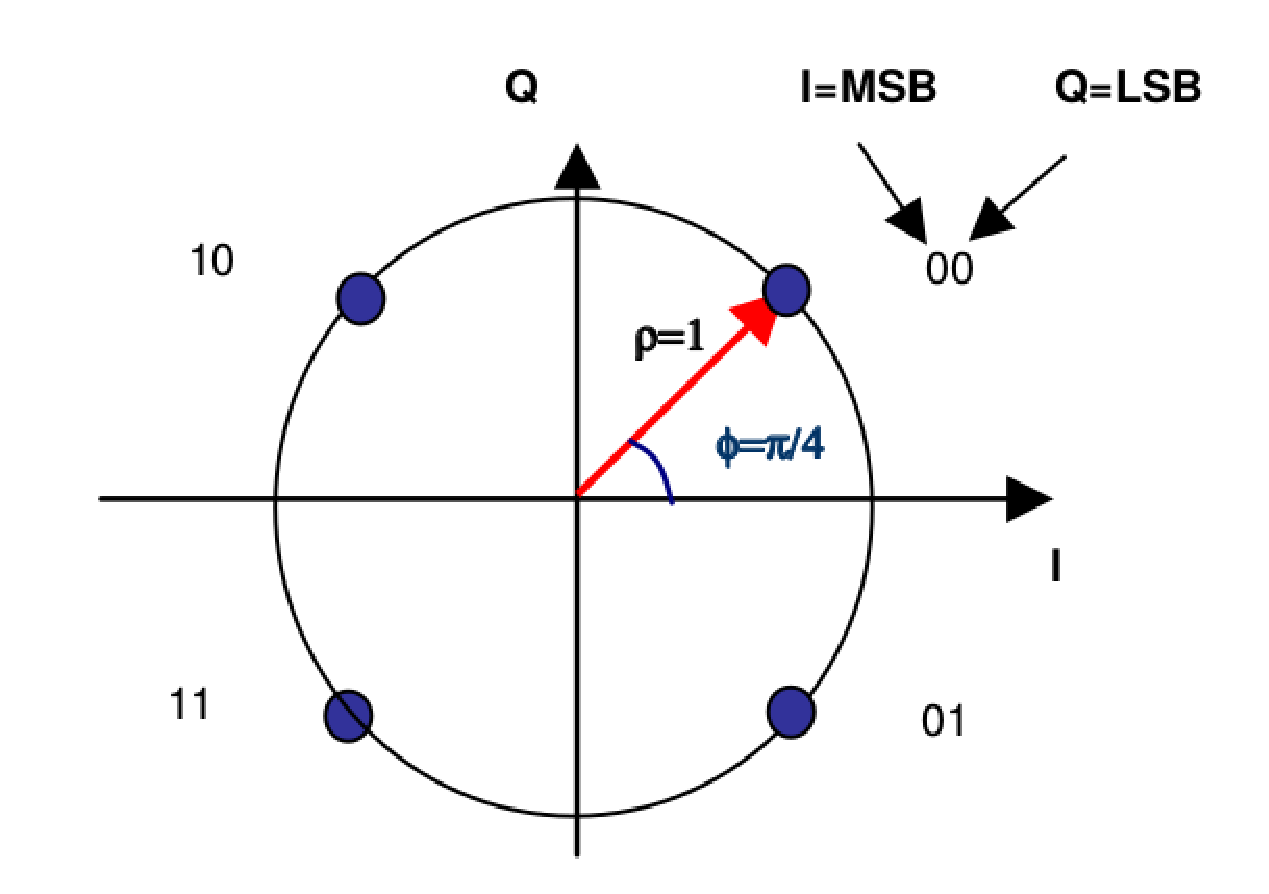
\includegraphics[width=\columnwidth]{./figs/qpsk}
\end{center}
\caption{Constellation diagram of QPSK}
\label{fig:qpsk}
\end{figure}
%------------------------------------------------------------------------------
% QSPK
%\begin{figure}
%\begin{tikzpicture}
%\draw[thick](0,0) circle (1);
%\filldraw [blue] (0.707106781,0.707106781) circle (2pt) node[anchor=west] {00};
%\filldraw [blue] (-0.707106781,0.707106781) circle (2pt) node[anchor=east] {10};
%\filldraw [blue] (-0.707106781,-0.707106781) circle (2pt) node[anchor=east] {11};
%\filldraw [blue] (0.707106781,-0.707106781) circle (2pt) node[anchor=west] {01};


%\draw[red,ultra thick,->] (0,0) -- (0.707106781,0.707106781);

%\draw[black,very thick,->] (-2,0) -- (2,0) node[anchor=west] {I};
%\draw[black,very thick,->] (0,-2) -- (0,2) node[anchor=east] {Q};

%\end{tikzpicture}
%\end{figure}

Demapping can be done by using,
\begin{align}
\frac{2\pi }{4}i < \angle{Y_k} < \frac{2\pi }{4}(i+1) \implies \hat{X_k}=X_i \quad i=0,\dots,3
\end{align}
%
Fig. \ref{fig:qpsk} Shows the Constellation mapping for QPSK scheme and similarly 

\subsection{8PSK}
Constellation Mapping symbol set $\cbrak{X}$ is generated by
\begin{equation}
X_k \in \cbrak{e^{j \frac{2\pi n}{8}}} \quad n=0,1,\dots,7
\end{equation}
\begin{figure}[!ht]
\begin{center}
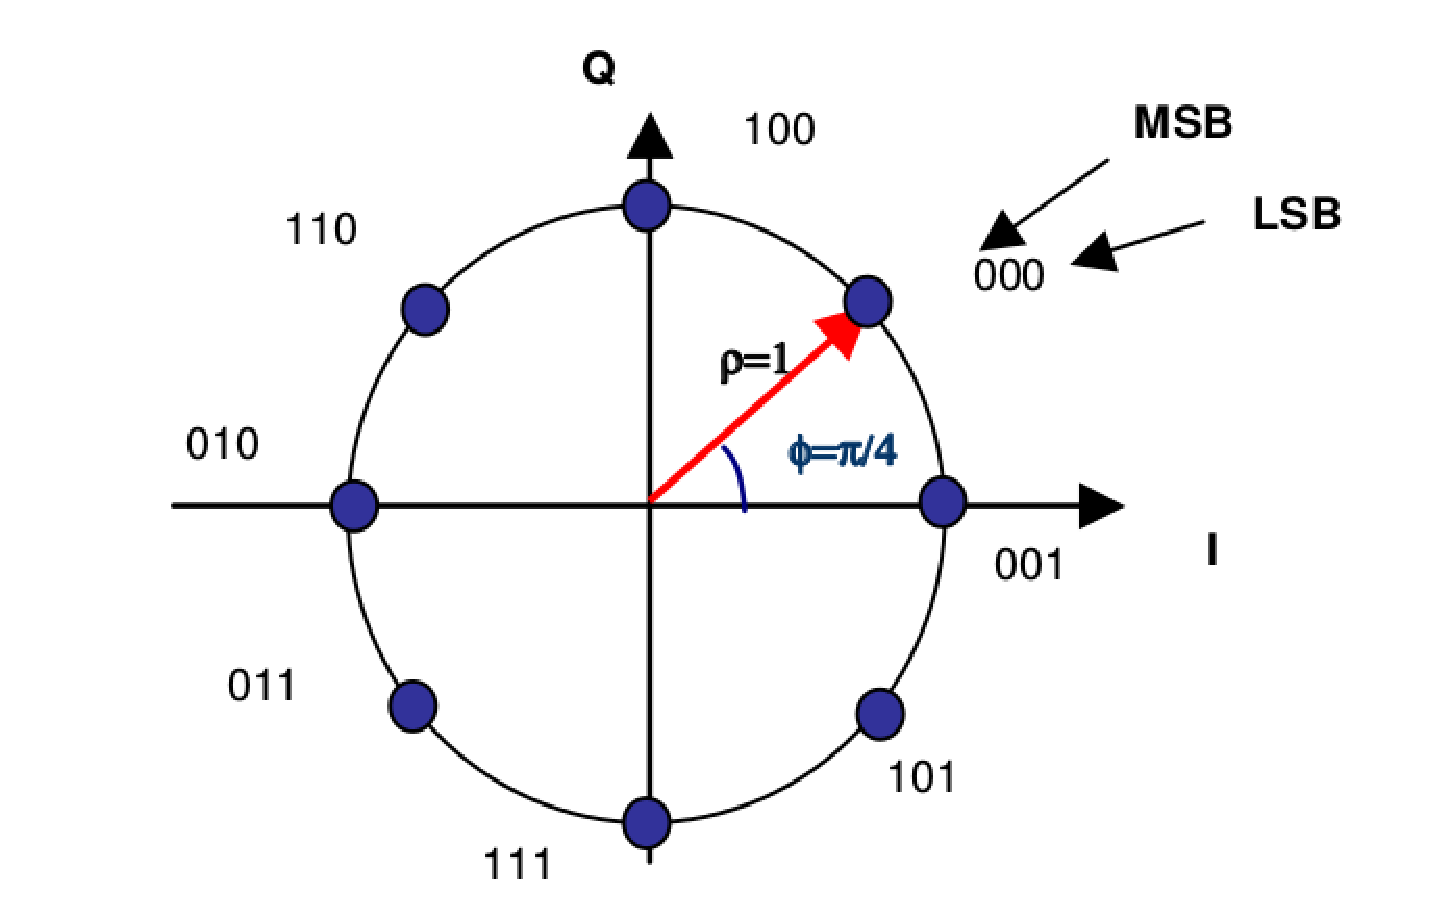
\includegraphics[width=\columnwidth]{./figs/8psk}
\end{center}
\caption{Constellation diagram of 8-PSK}
\label{fig:8psk}
\end{figure}
Demapping can be done by using,
\begin{align}
\frac{2\pi }{8}i < \angle{Y_k} < \frac{2\pi }{8}(i+1) \implies \hat{X_k}=X_i \quad i=0,\dots,7
\end{align}
Fig. \ref{fig:8psk} Shows the Constellation mapping for 8-PSK symbols and 
%
\section{Amplitude Phase Shift Keying (APSK)}

\subsection{16-APSK}
Constellation Mapping symbol set $\cbrak{X}$ is generated by
\begin{equation}
X_k \in \cbrak{X}=
\begin{cases}
r_1 e^{j\brak{\phi_1+\frac{2\pi}{4}n}}& n=0,\dots,3\\
r_2 e^{j\brak{\phi_2+\frac{2\pi}{12}n}}& n=0,1,\dots,11
\end{cases}
\end{equation}

Demapping can be done by using,
\begin{align}
\abs{Y_k}<\frac{r_1+r_2}{2} \&\& & \frac{2\pi }{4}i < \angle{Y_k} < \frac{2\pi }{4}(i+1)\\
& \implies \hat{X_k}=X_i \quad i=0,\dots,3\\
\abs{Y_k}>\frac{r_1+r_2}{2} \&\& & \frac{2\pi }{12}i < \angle{Y_k} < \frac{2\pi }{12}(i+1)\\
& \implies \hat{X_k}=X_i \quad i=4,\dots,15
\end{align}
Where $\frac{r_2}{r_1}=2.6$,$\phi_1=45,\phi_2=15$
Fig. \ref{fig:16apsk} Shows the Constellation mapping for 16-APSK symbols and  Fig. \ref{fig:16apsk1} Shows the Simulation diagram.
%
\begin{figure}[!ht]
\begin{center}
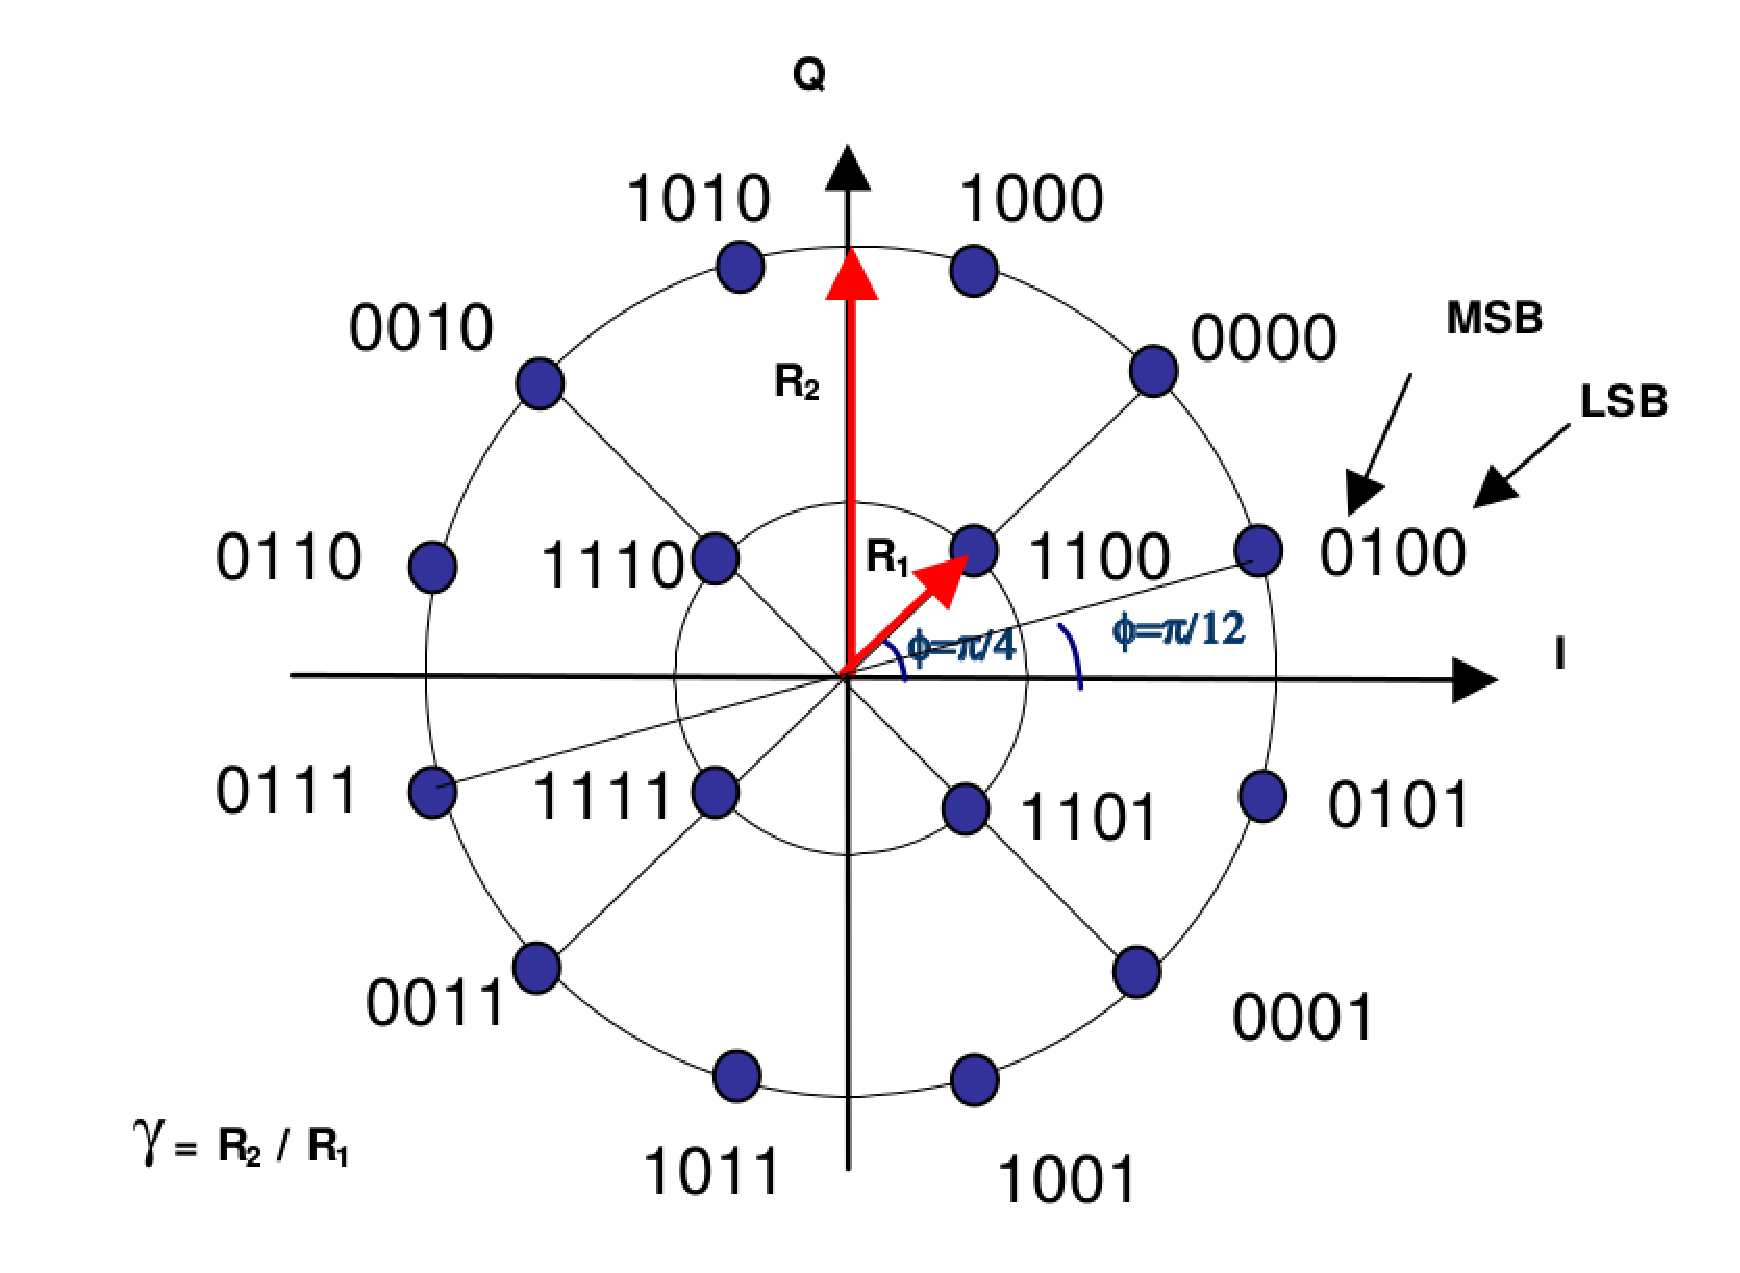
\includegraphics[width=\columnwidth]{./figs/16apsk}
\end{center}
\caption{Constellation diagram of 16APSK}
\label{fig:16apsk}
\end{figure}
%
\begin{figure}[!ht]
\begin{center}
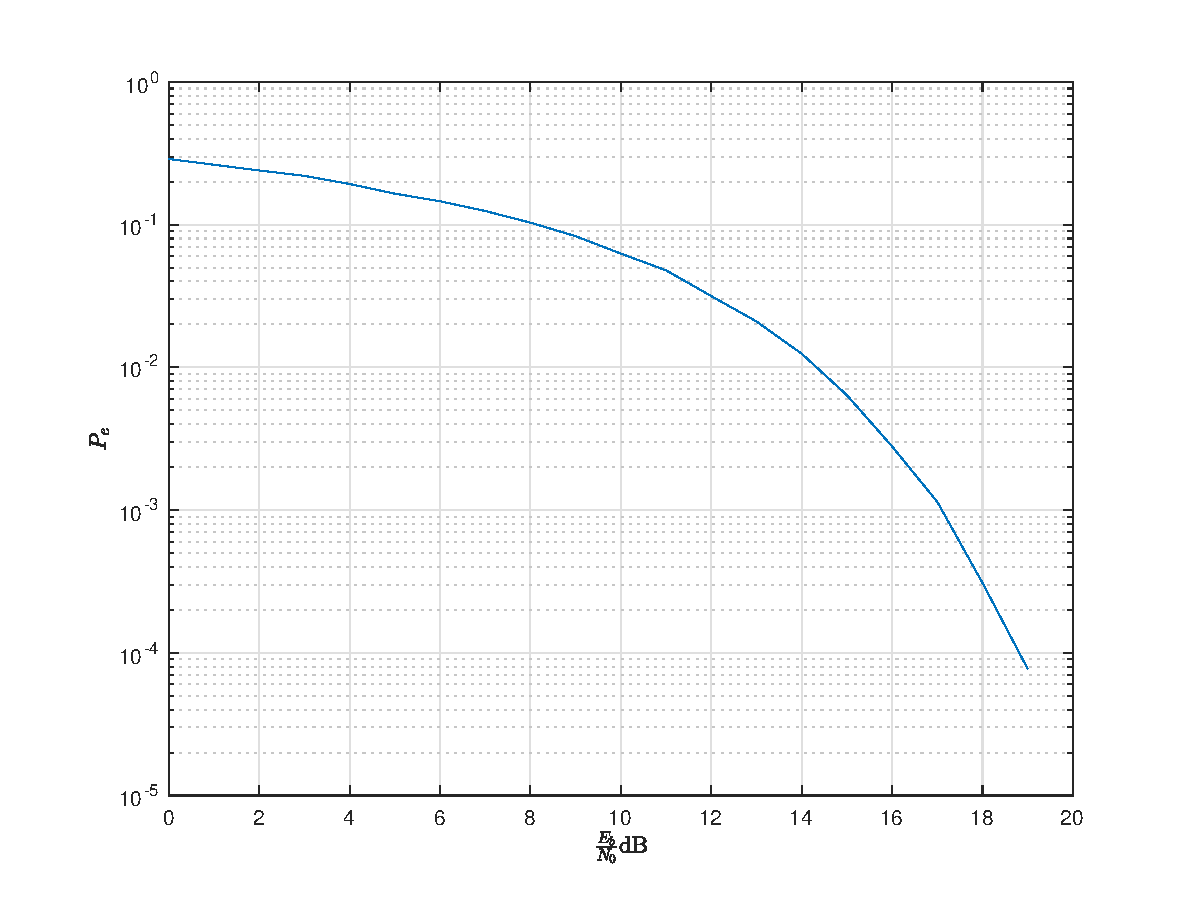
\includegraphics[width=\columnwidth]{./figs/apsk16}
\end{center}
\caption{SNR vs BER for 16-APSK}
\label{fig:16apsk1}
\end{figure}
%
\subsection{32-APSK}
Constellation Mapping symbol set $\cbrak{X}$ is generated by
\begin{equation}
X_k \in \cbrak{X}=
\begin{cases}
r_1 e^{j\brak{\phi_1+\frac{2\pi}{4}n}}& n=0,\dots,3\\
r_2 e^{j\brak{\phi_2+\frac{2\pi}{12}n}}& n=0,1,\dots,11\\
r_3 e^{j\brak{\phi_3+\frac{2\pi}{16}n}}& n=0,1,\dots,16
\end{cases}
\end{equation}
Where $\frac{r_2}{r_1}=2.54$,$\frac{r_3}{r_2}=4.33$,,$\phi_1=45,\phi_2=15,\phi_3=0$.

Demapping can be done by using,
\begin{align}
\abs{Y_k}<\frac{r_1+r_2}{2} \&\& & \frac{2\pi }{4}i < \angle{Y_k} < \frac{2\pi }{4}(i+1)\\
& \implies \hat{X_k}=X_i \quad i=0,\dots,3\\
\frac{r_1+r_2}{2}<\abs{Y_k}<\frac{r_2+r_3}{2} \&\& & \frac{2\pi }{12}i < \angle{Y_k} < \frac{2\pi }{12}(i+1)\\
& \implies \hat{X_k}=X_i \quad i=4,\dots,15 \\ 
\abs{Y_k}>\frac{r_2+r_3}{2} \&\& & \frac{2\pi }{12}i < \angle{Y_k} < \frac{2\pi }{12}(i+1)\\
& \implies \hat{X_k}=X_i \quad i=16,\dots,31
\end{align}

\begin{figure}[!ht]
\begin{center}
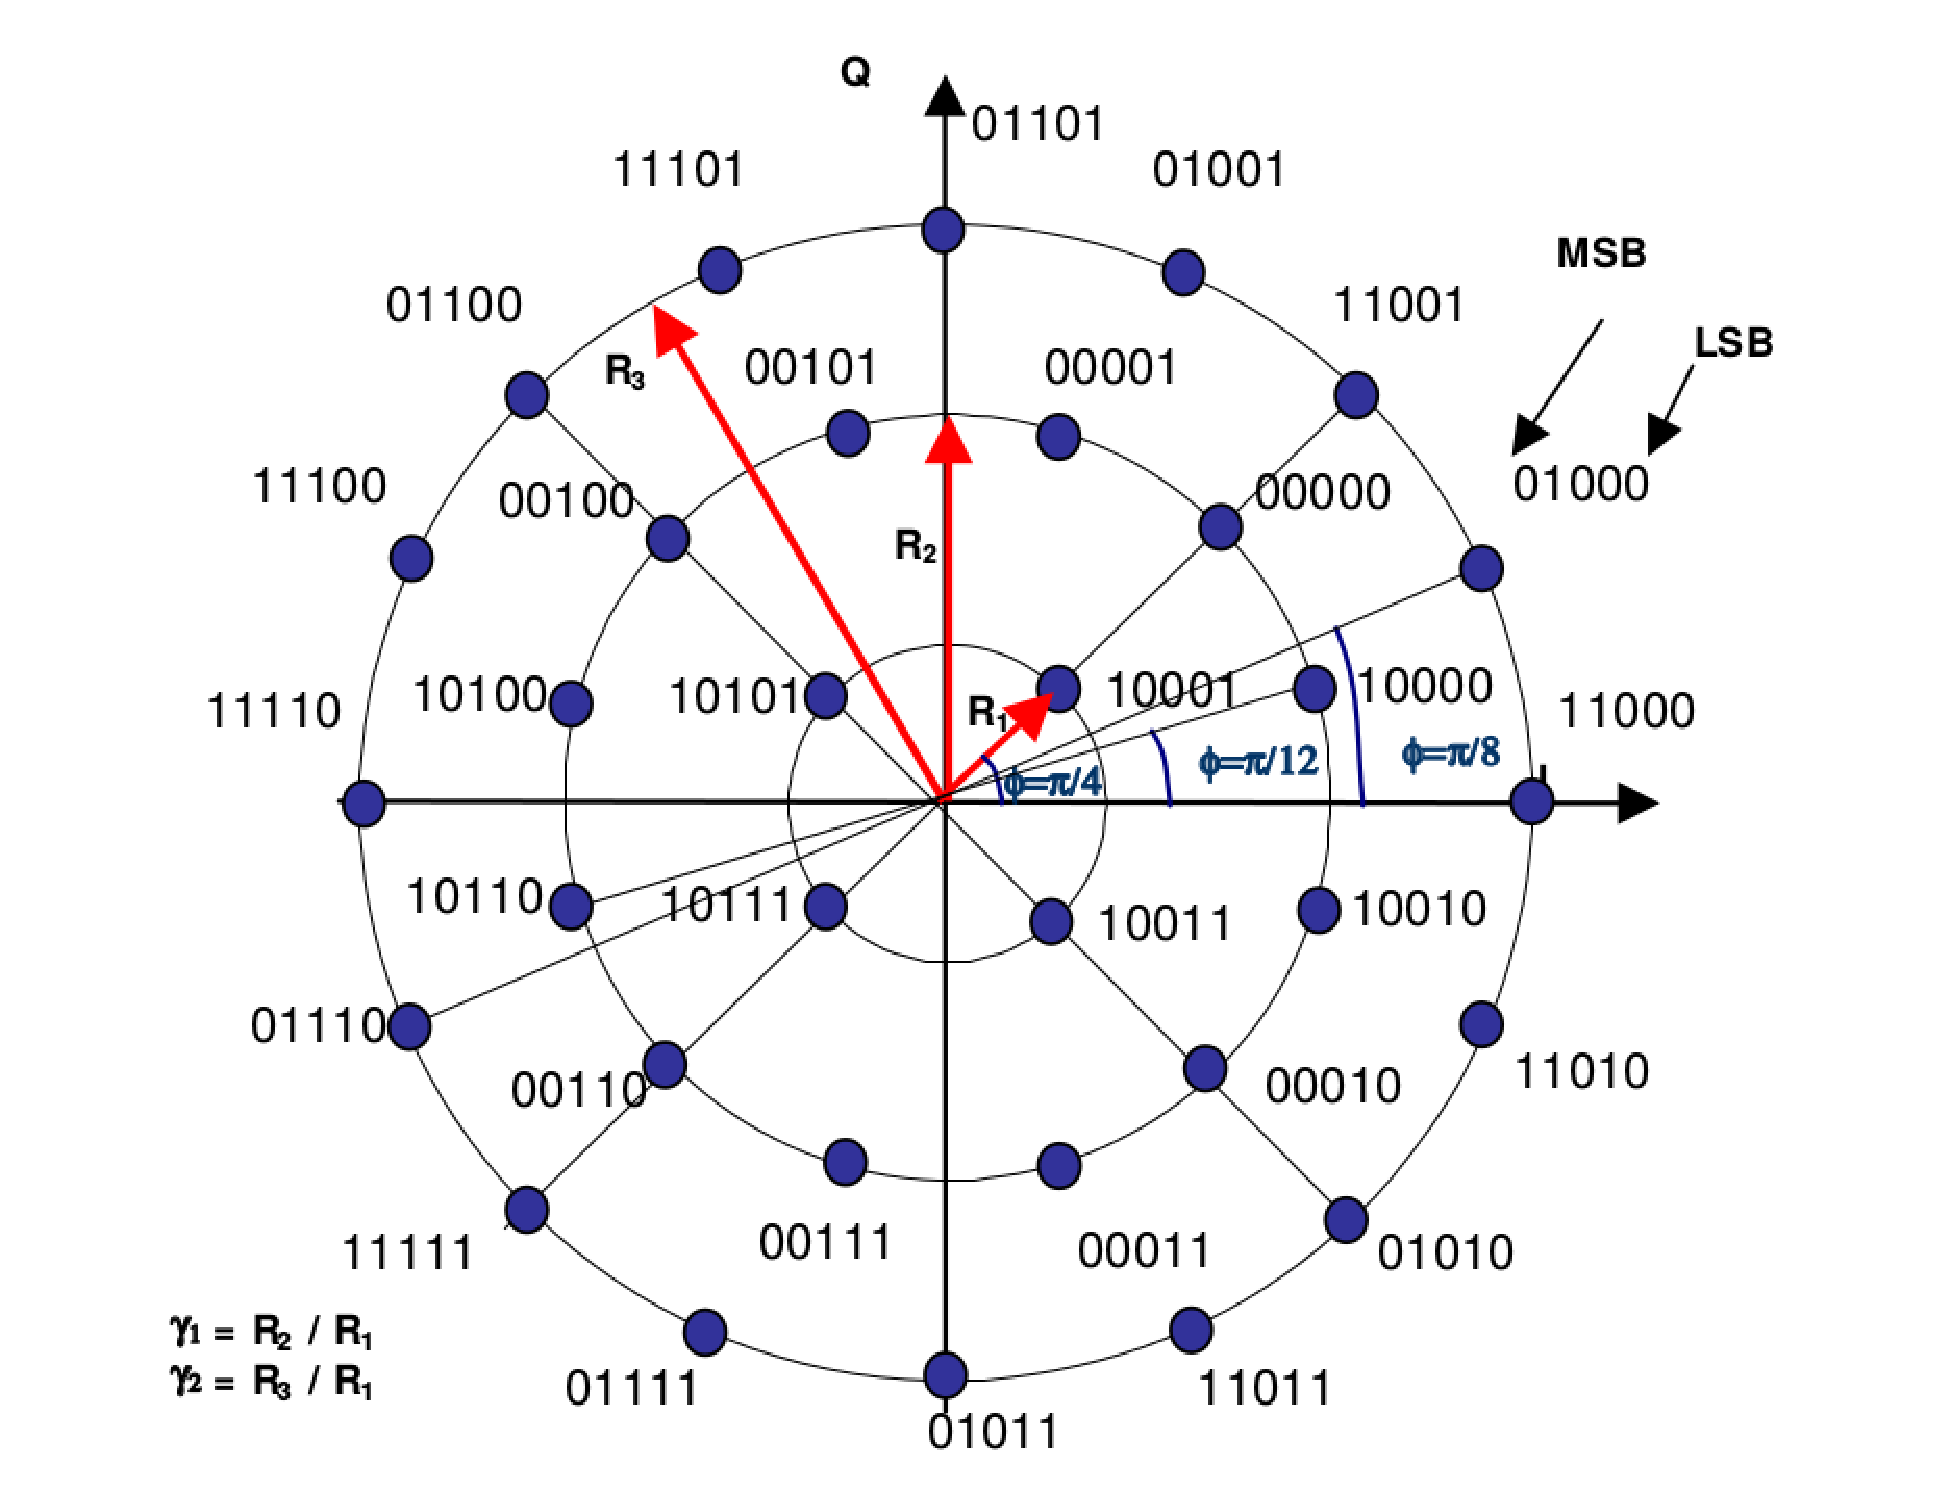
\includegraphics[width=\columnwidth]{./figs/32APSK}
\end{center}
\caption{Constellation diagram of 32APSK}
\label{fig:32apsk}
\end{figure}
Fig. \ref{fig:32apsk} shows the Constellation mapping for 32-APSK symbols and  Fig. \ref{fig:32apsk1} shows the Simulation diagram.

\begin{figure}[!ht]
\begin{center}
\includegraphics[width=\columnwidth]{./figs/apsk32}
\end{center}
\caption{SNR vs BER for 32-APSK}
\label{fig:32apsk1}
\end{figure}

\section{BCH: Generator Polynomial}
%\begin{enumerate}[label=\thesection.\arabic*
%,ref=\thesection.\theenumi]
For a BCH code, the minimal polynomials are given by 
\begin{align}
g_1(x)&=1+x+x^3+x^5+x^{14}\\
g_2(x)&=1+x^6+x^8+x^{11}+x^{14}\\
g_3(x)&=1+x+x^2+x^6+x^9+x^{10}+x^{14}\\
g_4(x)&=1+x^4+x^7+x^8+x^10+x^{12}+x^{14}\\
g_5(x)&=1+x^2+x^4+x^6+x^8+x^9+x^{11}
\nonumber \\
&\,+x^{13}+x^{14}\\
g_6(x)&=1+x^3+x^7+x^8+x^9+x^{13}+x^{14}\\
g_7(x)&=1+x^2+x^5+x^6+x^7+x^{10}+x^{11}
\nonumber \\
&\,+x^{13}+x^{14}\\
g_8(x)&=1+x^5+x^8+x^9+x^{10}+x^{11}+x^{14}\\
g_9(x)&=1+x+x^2+x^3+x^9+x^{10}+x^{14}\\
g_{10}(x)&=1+x^3+x^6+x^9+x^{11}+x^{12}+x^{14}\\
g_{11}(x)&=1+x^4+x^{11}+x^{12}+x^{14}\\
g_{12}(x)&=1+x+x^2+x^3+x^5+x^6+x^7+x^8
\nonumber \\
&\,+x^{10}+x^{13}+x^{14}
\end{align}
The generator polynomial is obtained as
\begin{align}
g(x) =\prod_{i = 1}^{m}g_i(x)
\end{align}

%where $m=12$.
%maximum number of errors that can be corrected by $\vec{g}$ is $m = 12$.

%\end{enumerate}
\section{BCH: Encoding}
%\begin{enumerate}[label=\thesection.\arabic*
%,ref=\thesection.\theenumi]
 Let $\vec{m}$ be a $k \times 1$ message vector and  
\begin{equation}
m(x)=m_{k-1}x^{k-1}+m_{k-2}x^{k-2}+\dots+m_1x+m_0
\end{equation} 
be the  corresponding Message polynomial. 
%\begin{equation}
%g(x)=g_{n-k}x^{n-k}+g_{n-k-1}x^{n-k-1}+\dots+g_1x+g_0
%\end{equation}
%be the Generator polynomial.
%\item Multiply the message polynomial $m(x)$ by $x^{n-k}$, then the message polynomial becomes,
%\begin{equation}
%m(x)x^{n-k}=m_{n-1}x^{n-1}+m_{n-2}x^{n-2}+\dots+m_1x+m_0
%\end{equation}
Let 
\begin{equation}
m(x)x^{n-k} = q(x)g(x)+d(x)
\end{equation} 
and 
\begin{equation}
c(x)=m(x)x^{n-k}+d(x)
\end{equation}
%

%\end{enumerate}
\section{Berlekamp's Decoding Algorithm}
%\begin{enumerate}[label=\thesection.\arabic*
%,ref=\thesection.\theenumi]

Let $\vec{\alpha}_i, 2 \le i \le 2m+1$ be the $i$th row of $\vec{A}$ and $\alpha_i(x)$ be the
corresponding polynomial. Let $\vec{r}$ be the received codeword (noisy). $r(x)$ is then defined to be the 
received polynomial.the correspondig syndromes. 

\begin{equation}
S_i(x) = r\brak{\alpha_i(x)}
\end{equation}

 Intialization : $k=0, \Lambda^{(0)}(x)=1,T^{(0)}=1$
 Let $\Delta^{(2k)}$ be the coefficient of $x^{2k+1}$ in $\Lambda^{(2k)}[1+S(x)]$ 
 Compute  
\begin{equation}
\Delta^{(2k+2)}(x)=\Lambda^{(2k)}(x) +\Delta^{(2k)}[x.T^{(2k)}(x)]
\end{equation}
 Compute \begin{equation}
    	T^{(2k+2)}(x) =
    \begin{cases}
    	x^2T^{(2k)}(x) & \text{if $\Delta^{(2k)}=0$ or deg}\sbrak{\Lambda^{(2k)}(x)}>k\\
      \frac{x \Lambda^{(2k)}(x)}{\Delta^{(2k)}} & \text{if $\Delta^{(2k)}\neq 0$ or 
deg}\sbrak{\Lambda^{(2k)}(x)}\leq k
    \end{cases}
  \end{equation}
 Set $k=k+1$.If $k<t$ then go to step3.
 Return the Error Locator polynomial $\Lambda(x)=\Lambda^{(2k)}(x)$

\section{BCH Decoding: The Chien's Search Algorithm}
\begin{enumerate}[label=\thesection.\arabic*
,ref=\thesection.\theenumi]
\item Take $\alpha ^j$ as test root . $0\leq j \leq n-1$.
\item if $\Lambda_i $ test every root and if its equals to zero. Then that is root.
\item  Flip the bit values at root positions.
\item Let the Received polynomial be $r(x)$ i.e which contains both transmitted codeword polynomial $c(x)$ and 
the 
error polynomial $e(x)$ \begin{equation}
e(x)=e_0+e_1x^1+...+e_{n-1}x^{n-1}
\end{equation} Where $e_i$ represents the value of the error at the location. For binary BCH codes  $e_i$ is 
either 0 or 1.
\begin{equation}
r(x)=c(x)+e(x)=r_{n-1}x^{n-1}+r_{n-2}x^{n-2}+\dots+r_1x+r_0
\end{equation}
Definie, Syndrome \begin{equation}
S_i=r(\alpha^i)=c(\alpha^i)+e(\alpha^i)=e(\alpha^i)
\end{equation} Where $\alpha^i $ is a root of the codeword.
Suppose that $v$ errors occurred, and $0\leq v \leq t$.
Let the error occurs at $i_1,i_2,\dots,i_v$. 
The Decoding Process, for a t-error correcting code will follows the basic steps,
\end{enumerate}

\section{LDPC: Introduction}
Let the Channel model be,
\begin{equation}
Y_k= X_k + V_k, \quad k = 0,\dots,6
\end{equation} 
where $X_k$ is the  transmitted symbol in the $k$th time slot using the BPSK modulation and $V_k \sim \mathcal{N}\brak{0,\sigma^2} $. 

\section{LDPC: Encoding}
 LDPC codes are popular linear block codes with closest Shannon limit channel capacity \cite{ldpc}. As an example, lets take (7,4) Hamming parity check matrix.
 \begin{equation} \label{eq:H}
 H =  \begin{bmatrix} 
1 & 1 & 1 & 0 & 1 & 0 & 0 \\
1 & 0 & 1 & 1 & 0 & 1 & 0 \\
1 & 1 & 0 & 1 & 0 & 0 & 1 
\end{bmatrix}
 \end{equation}

%The above $H$ matrix has $k=4$ i.e $\vec{m}=\myvec{m_0 &\dots & m_3}$ information bits  and $m=n-k=3$ i.e $\vec{p}=\myvec{p_0 &p_1 &p_2}$ parity bits. The code word length $n=7$ i.e $\vec{c}=\myvec{\vec{m} & \vec{p}}$.
\begin{figure}[!ht]
\begin{center}
%\begin{tikzpicture}
%
%    \node[shape=circle,draw=black] (v6) at (0,0) {v6};
%    \node[shape=circle,draw=black] (v5) at (0,1) {v5};
%    \node[shape=circle,draw=black] (v4) at (0,2) {v4};
%    \node[shape=circle,draw=black] (v3) at (0,3) {v3};
%    \node[shape=circle,draw=black] (v2) at (0,4) {v2};
%    \node[shape=circle,draw=black] (v1) at (0,5) {v1};
%    \node[shape=circle,draw=black] (v0) at (0,6) {v0};
%
%    
%
%
%    \node[shape=rectangle,draw=black] (p0) at (4,5) {p0};
%    \node[shape=rectangle,draw=black] (p1) at (4,3) {p1};
%    \node[shape=rectangle,draw=black] (p2) at (4,1) {p2};
%
%\path [-] (v0) edge node[left] {} (p0);
%\path [-] (v0) edge node[left] {} (p1);
%\path [-] (v0) edge node[left] {} (p2);
%\path [-] (v1) edge node[left] {} (p0);
%\path [-] (v1) edge node[left] {} (p2);
%\path [-] (v2) edge node[left] {} (p0);
%\path [-] (v2) edge node[left] {} (p1);
%\path [-] (v3) edge node[left] {} (p1);
%\path [-] (v3) edge node[left] {} (p2);
%\path [-] (v4) edge node[left] {} (p0);
%\path [-] (v5) edge node[left] {} (p1);
%\path [-] (v6) edge node[left] {} (p2);
%
%\path [->] (-1,0) edge node[left] {} (v6);
%\path [->] (-1,1) edge node[left] {} (v5);
%\path [->] (-1,2) edge node[left] {} (v4);
%\path [->] (-1,3) edge node[left] {} (v3);
%\path [->] (-1,4) edge node[left] {} (v2);
%\path [->] (-1,5) edge node[left] {} (v1);
%\path [->] (-1,6) edge node[left] {} (v0);
%
%\node[] at (-1.7,0) {$L(6)$};
%\node[] at (-1.7,1) {$L(5)$};
%\node[] at (-1.7,2) {$L(4)$};
%\node[] at (-1.7,3) {$L(3)$};
%\node[] at (-1.7,4) {$L(2)$};
%\node[] at (-1.7,5) {$L(1)$};
%\node[] at (-1.7,6) {$L(0)$};
%
%\node[] at (0,7) {variable nodes};\\
%\node[] at (4,7) {check nodes};\\
%\end{tikzpicture}
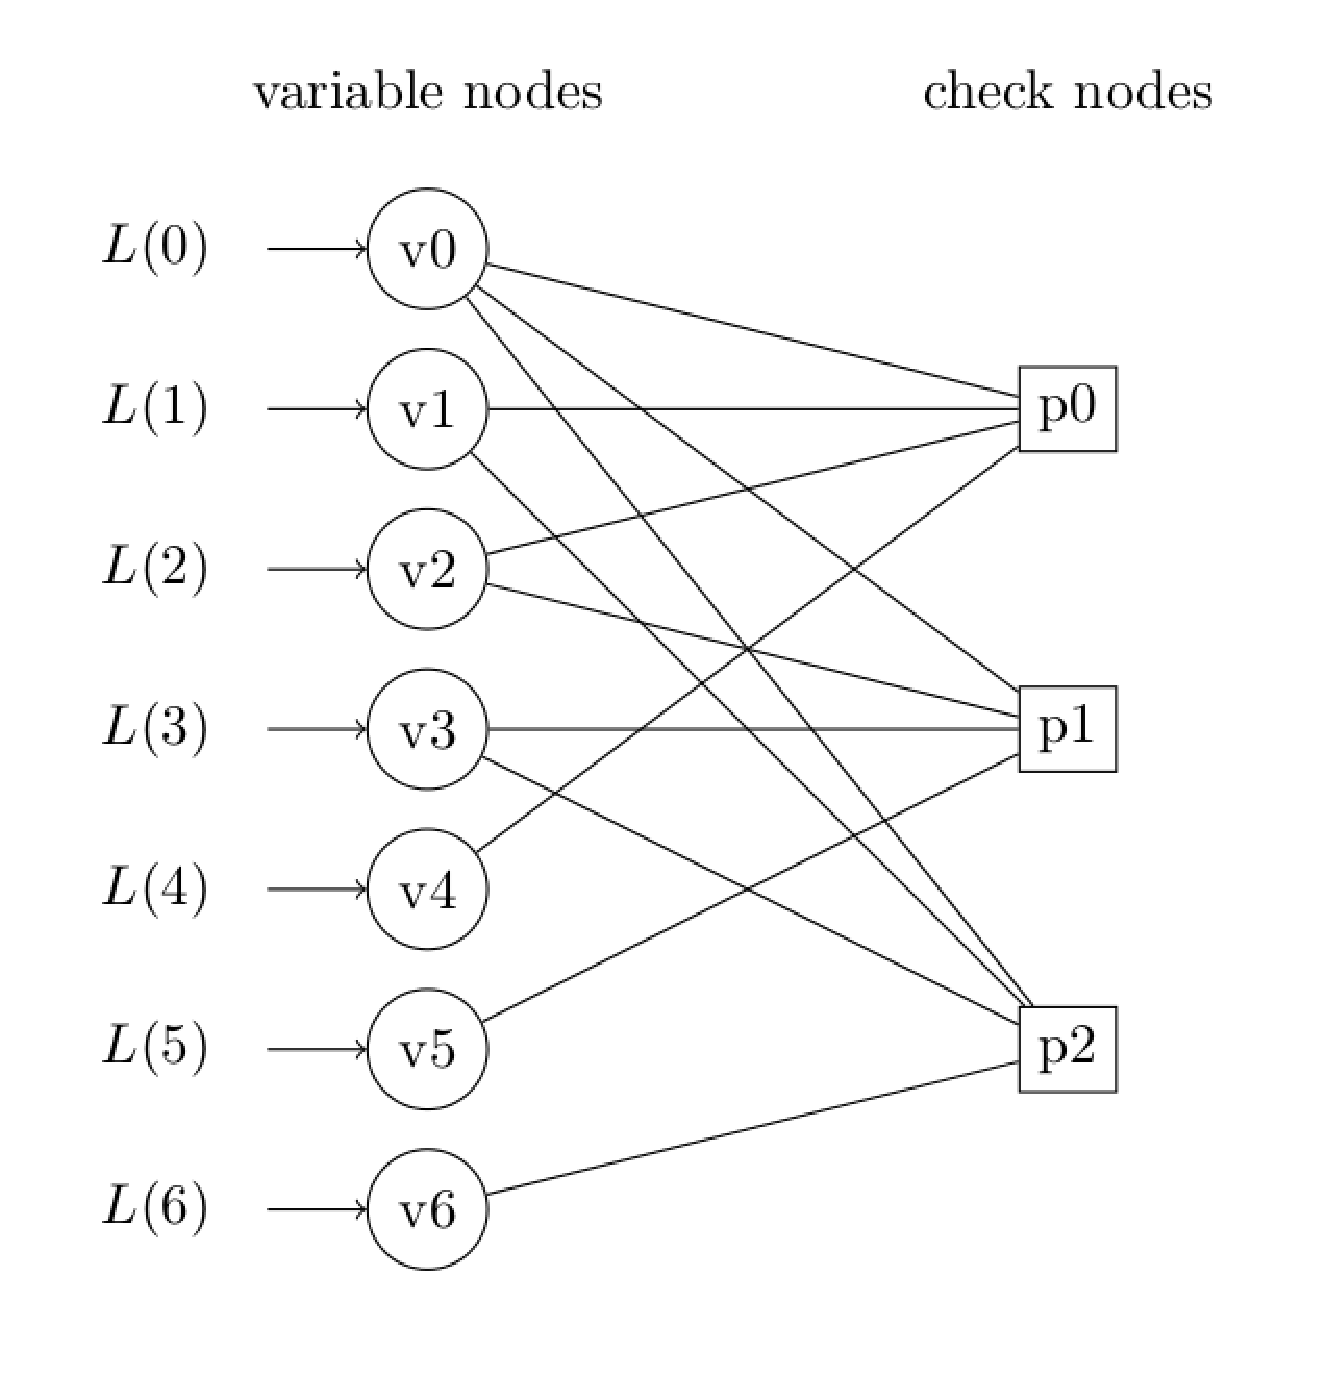
\includegraphics[width=\columnwidth]{./figs/tanner}
\caption{Tanner Graph Representation for (7,4) Hamming parity check matrix}
\label{fig:tanner}
\end{center}
\end{figure}
Encoding can be carried out by using 
\begin{align}
H &\times c^T =0 \\
 \begin{bmatrix} 
1 & 1 & 1 & 0 & 1 & 0 & 0 \\
1 & 0 & 1 & 1 & 0 & 1 & 0 \\
1 & 1 & 0 & 1 & 0 & 0 & 1 
\end{bmatrix} &  \begin{bmatrix} 
m_0\\
m_1\\
m_2\\
m_3 \\
p_0 \\
p_1\\
p_2
\end{bmatrix} = 0
\end{align}
solving we get
\begin{align}
p_0 &= m_0 \oplus m_1 \oplus m_2 \\
p_1 &= m_0 \oplus m_2 \oplus m_3 \\
p_2 &= m_0 \oplus m_1 \oplus m_3 
\end{align}
This is called Systematic Encoding.i.e Encoder will ensures information bits followed by parity bits.
\section{LDPC: Decoding}
\subsection{Useful Calculations for proceeding LDPC Decoding }
\begin{enumerate}
\item Calculation of Input Channel Log Likelihood Ratio LLR 
\begin{align}
L(x_j)&=\log \brak{\frac{Pr(x_j=1|y)}{Pr(x_j=-1|y)}} \quad X=1-2c\\
&= \log \brak{\frac{f(y|x_j=1)Pr(x_j=1)}{f(y|x_j=-1)Pr(x_j=-1)}} \\
&= \log \brak{\frac{\frac{1}{\sqrt{2\pi\sigma^2}}e^{\frac{-(y_j-1)^2}{2\sigma^2}}}{\frac{1}{\sqrt{2\pi\sigma^2}}e ^{\frac{-(y_j+1)^2}{2\sigma^2}}} } \\
&=\log \brak{e^{\frac{2y_j}{\sigma^2}}} \\
L(x_j)&= \frac{2y_j}{\sigma^2} \label{eq :li}
\end{align}
\item Check Node Operation : \\
Lets assume that we have initilized all LLR values to variable nodes and we sent to check nodes. ${V_j}$ represents all the variable nodes which are connected to $j^{th}$ check node. Using the min-sum approximation\cite{minsum}, the message from  $j^{th}$ check node to  $i^{th}$ variable node given by,
\begin{figure}[!ht]
\begin{center}
%\begin{tikzpicture}
%    \node[shape=circle,draw=black] (v4) at (0,3) {v4};
%
%    \node[shape=circle,draw=black] (v2) at (0,4) {v2};
%    \node[shape=circle,draw=black] (v1) at (0,5) {v1};
%    \node[shape=circle,draw=black] (v0) at (0,6) {v0};
%
%    \node[shape=rectangle,draw=black] (p0) at (3,5) {p0};
%
%\path [<-] (v0) edge node[left] {} (p0);
%
%\path [->] (v1) edge node[left] {} (p0);
%
%\path [->] (v2) edge node[left] {} (p0);
%
%\path [->] (v4) edge node[left] {} (p0);
%
%
%
%\path [->] (-1,3) edge node[left] {} (v4);
%\path [->] (-1,4) edge node[left] {} (v2);
%\path [->] (-1,5) edge node[left] {} (v1);
%\path [->] (-1,6) edge node[left] {} (v0);
%
%
%\node[] at (-1.7,3) {$L(4)$};
%\node[] at (-1.7,4) {$L(2)$};
%\node[] at (-1.7,5) {$L(1)$};
%\node[] at (-1.7,6) {$L(0)$};
%
%
%\end{tikzpicture}
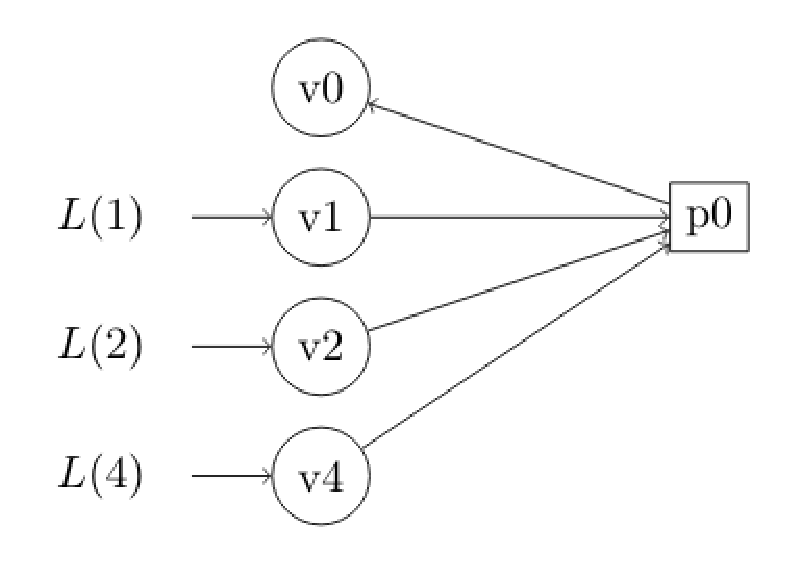
\includegraphics[width=\columnwidth]{./figs/checkope}
\end{center}
\caption{Check node operation}
\label{fig : check}
\end{figure}
since parity node equation for the first check node is $p_0=m_0+m_1+m_2+m_4$. we need to calculate
\begin{align}
L_{ext0,0} &= \log \brak{\frac{Pr(x_0 =0 | y_1,y_2,y_4)}{Pr(x_0 =1| y_1,y_2,y_4)}}
\end{align}
Defining,
\begin{align}
L_1 &= \log \brak{\frac{Pr(x_1 =0 | y_1)}{Pr(x_1 =1| y_1)}} = \log \brak{\frac{p_1}{1-p_1}} \\
L_2 &= \log \brak{\frac{Pr(x_2 =0 | y_2)}{Pr(x_2 =1| y_2)}}=\log \brak{\frac{p_2}{1-p_2}} \\
L_4 &= \log \brak{\frac{Pr(x_4 =0 | y_4)}{Pr(x_4 =1| y_4)}}= \log \brak{\frac{p_4}{1-p_4}} \\
\end{align}
\begin{table}[!ht]
\begin{center}
{\tiny
\input{./figs/ptable.tex}
}
\end{center}
\caption{Probability of a varibale node from other check nodes}
\label{table:type}
\end{table}
Using Table. \ref{table:type} we can find the 
\begin{equation}
p_0=Pr(c_0=0|c_1,c_2,c_4)
\end{equation}
\begin{align*}
p_0 &= p_1p_2p_4 + p_1(1-p_2)(1-p_4)\\
&+(1-p_1)p_2(1-p_4)
+(1-p_1)(1-p_2)p_4\\
1-p_0 &=p_1p_2(1-p_4) + p_1(1-p_2)p_4\\
&+(1-p_1)p_2p_4+(1-p_1)(1-p_2)(1-p_4)\\
\end{align*}
by rearranging above equations,
\begin{equation}
p_0 - (1-p_0) = p_1 -(1-p_1) + p_2 - (1-p_2) + p_4 -(1- p_4)
\end{equation}
%\begin{equation}\label{eq:sub}
%\log \brak{\frac{1-\frac{1-p_0}{p_0}}{1+\frac{1-p_0}{p_0}}}
%\end{equation}

Where $p_i$ is the probability. getting message from check to variable node by taking all variable node informations.
\begin{align}
\frac{1-\frac{1-p_0}{p_0}}{1+\frac{1-p_0}{p_0}} & = \frac{1-\frac{1-p_1}{p_1}}{1+\frac{1-p_1}{p_1}} \times \frac{1-\frac{1-p_2}{p_2}}{1+\frac{1-p_2}{p_2}} \times \frac{1-\frac{1-p_4}{p_4}}{1+\frac{1-p_4}{p_4}}\\
\frac{1-e^{-L_{ext0,0}}}{1+e^{-L_{ext0,0}}} &=\frac{1-e^{-L_{1}}}{1+e^{-L_{1}}}\times \frac{1-e^{-L_{2}}}{1+e^{-L_{2}}} \times \frac{1-e^{-L_{4}}}{1+e^{-L_{4}}}\\ \nonumber
-\tanh \brak{\frac{L_{ext0,0}}{2}}& =\brak{-\tanh \brak{\frac{L_{1}}{2}}}\brak{-\tanh \brak{\frac{L_{2}}{2}}}\\
&\brak{ -\tanh \brak{\frac{L_{4}}{2}} }
\end{align}
\begin{align}
L_{ext0,0}&=\brak{\prod_{k \in V_j \setminus i}\alpha_{k,0}} f\brak{\sum_{k \in V_j \setminus i}f\brak{\beta_{k,0}}} \label{eq:main}
\end{align}
Where,
\begin{align}
\alpha_{k,j}&=sign(L_{k,j})\\
\beta_{k,j}&=\abs{L_{k,j}}\\
f(x)&= - \log \brak{\tanh{\frac{x}{2}}}
\end{align}
 \begin{figure}[!ht]
\begin{center}
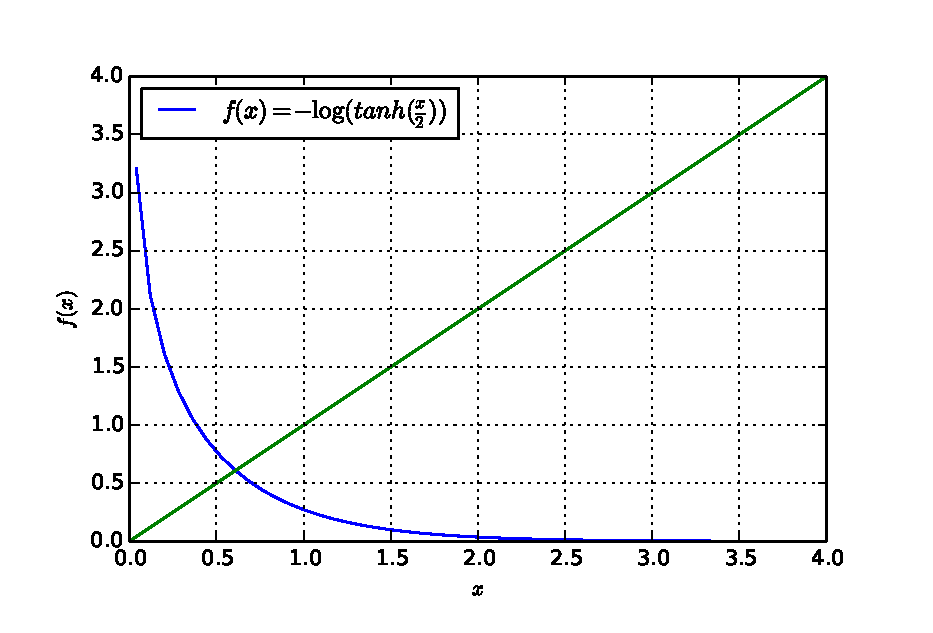
\includegraphics[width=\columnwidth]{./figs/fxgraph}
\caption{Plot of function $f(x)$}
\label{fig : fx}
\end{center}
\end{figure}
Using the Fig \ref{fig : fx} and using its $45^\circ$ symmetricity, we can approximate the above equation as, given by minimum sum approximation \cite{minsum} 
\begin{align}
f\brak{\sum_{k \in V_j \setminus i}f\brak{\beta_{k,0}}} &\approx f\brak{f\brak{\min_{k \in V_j \setminus i}\brak{\beta_{k,0}}}}\\
&=\min_{k \in V_j \setminus i}\brak{\beta_{k,0}} \label{eq: minsumapp}
\end{align}
Combining \eqref{eq: minsumapp} in \eqref{eq:main},
\begin{align}
L(r_{j=0,i=0}) &=\brak{\prod_{k \in V_j \setminus i}\alpha_{k,0}} \brak{\min_{k \in V_j \setminus i}\brak{\beta_{k,0}}} \label{eq:rji}
\end{align}
%
\item Variable Node Operation :\\
Let ${C_i}$ denotes all the check nodes connected to $i^{th}$ variable node. The message from $i^{th}$ variable node to  $j^{th}$ check node given by,
\begin{figure}[!ht]
\begin{center}
%\begin{tikzpicture}
%
%    
%    \node[shape=circle,draw=black] (v0) at (0,3) {v0};
%
%    
%
%
%    \node[shape=rectangle,draw=black] (p0) at (2,4) {p0};
%    \node[shape=rectangle,draw=black] (p1) at (2,3) {p1};
%    \node[shape=rectangle,draw=black] (p2) at (2,2) {p2};
%
%\path [->] (v0) edge node[left] {} (p0);
%\path [<-] (v0) edge node[left] {} (p1);
%\path [<-] (v0) edge node[left] {} (p2);
%
%
%\path [->] (-1,3) edge node[left] {} (v0);
%
%\node[] at (-1.4,3) {$L(0)$};
%
%\end{tikzpicture}
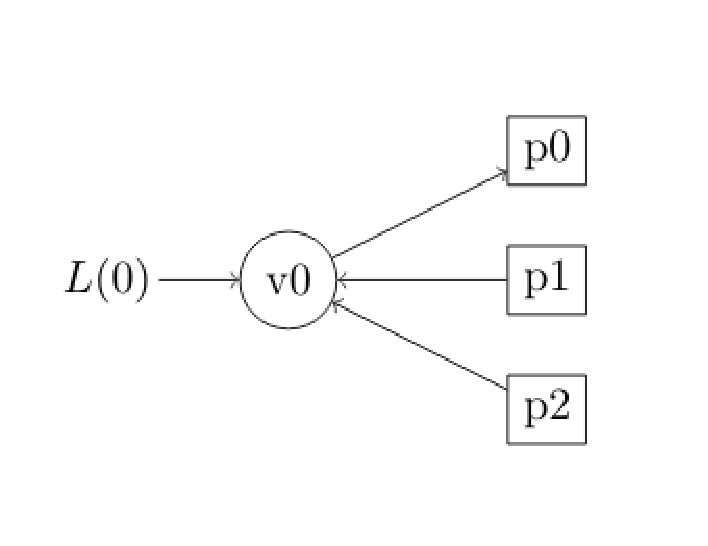
\includegraphics[width=\columnwidth]{./figs/varope}
\end{center}
\caption{Variable node operation}
\label{fig : var}
\end{figure}
\begin{align}
L(q_{i=0,j=0})&=\log \brak{\frac{Pr(x_j=1|y_0,y_1,y_2)}{Pr(x_j=-1|y_0,y_1,y_2)}} \quad X=1-2c\\
&= \log \brak{\frac{f(y_0,y1,y_2|x_j=1)Pr(x_j=1)}{f(y_0,y_1,y_2|x_j=-1)Pr(x_j=-1)}} \\
&= \log \brak{\frac{\brak{\frac{1}{\sqrt{2\pi\sigma^2}}}^3e^{\frac{-(y_0-1)^2}{2\sigma^2}}e^{\frac{-(y_1-1)^2}{2\sigma^2}}e^{\frac{-(y_2-1)^2}{2\sigma^2}}}{\brak{\frac{1}{\sqrt{2\pi\sigma^2}}}^3e ^{\frac{-(y_0+1)^2}{2\sigma^2}}e ^{\frac{-(y_1+1)^2}{2\sigma^2}}e ^{\frac{-(y_2+1)^2}{2\sigma^2}} }  } \\
&=\log \brak{e^{\frac{2(y_0+y_1+y_2)}{\sigma^2}}} \\
L(q_{i=0,j=0})&= \frac{2(y_0+y_1+y_2)}{\sigma^2}=L(x_i)+\sum_{k \in C_i\setminus j} L(r_{ki}) \label{eq: qij}
\end{align}
\end{enumerate}

\subsection{Message Passing Algorithm using min-sum Approximation}
Transmitted frames = N, Total number of bits = N $\times$ 7 and Total number of information bits = N $\times$ 4.
For Each Frame,
\begin{enumerate}
\item Initialize $L(q_{ij})$ using \eqref{eq :li} for all $i,j$ for which $h_{ij}=1$ with channel LLR's.
\item Update $\cbrak{L(r_{ji})}$ using \eqref{eq:rji}
\item Update $\cbrak{L(q_{ji})}$ using \eqref{eq: qij}.
\item Update $\cbrak{L(V_i)}$ using,
\begin{equation}
L(V_i)=L(x_i)+\sum_{k \in C_i} L(r_{ki}) \quad i=0,\dots,6.
\end{equation}
\item Proceed to step 2.\\
After maximum specified iterations,

\end{enumerate}
Decoding can be done using,
\begin{equation}
\hat{c_i} = \begin{cases}
1 & L(V_i) < 0\\
0 & else
\end{cases}
\end{equation}
%
\subsection{Simulation Results}
For frames N=10000.
 \begin{figure}[!ht]
\begin{center}
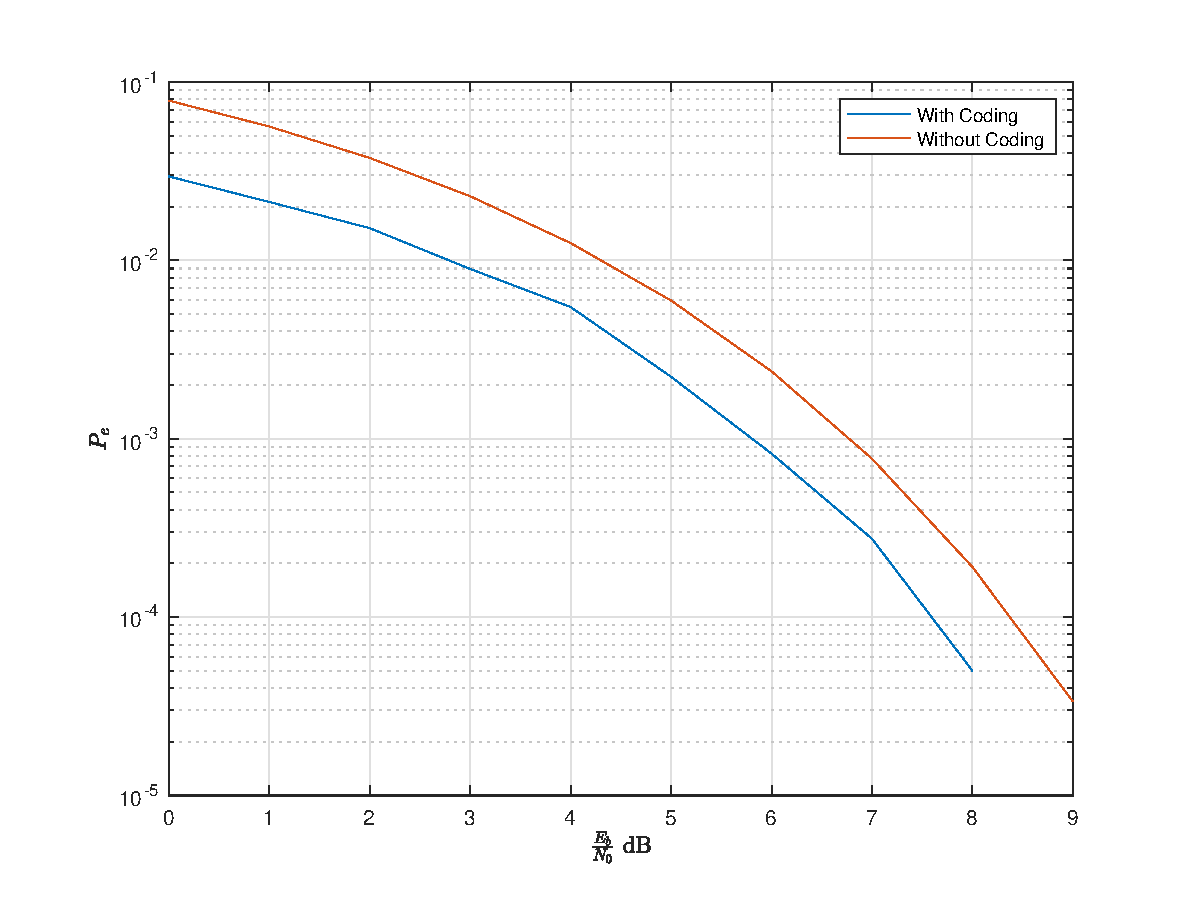
\includegraphics[width=\columnwidth]{./figs/ber}
\caption{SNR vs BER curves using LDPC channel coding and no channel coding}
\label{fig : ber}
\end{center}
\end{figure}
Fig \ref{fig : ber} Shows the Comparison of Probability error with channel coding and without channel coding. Since the parity check matrix taken was not much sparse, we are not getting near shannon limit performance. (Good sparse matrix i.e number of entries in H $<< m\times n $ )

\section{LDPC Decoding for Higher Order Mapping Schemes}
In the case of higher order mapping schemes, calculation of Log Likelihood Ratio's are crutial. A generalized and approximated Log Likelihood Ratio given by \cite{llr}
\subsection{General Expression for Calculation of Log Likelihood Ratio(LLR)}
\begin{align}
LLR(b_j)&= \log \brak{\frac{Pr(b_j=0|y)}{Pr(b_j=1|y)}}\\
LLR(b_j)&=\log \brak{\frac{\sum_{i\in \cbrak{K_{b_j=0}}}\frac{1}{2\sigma^2}e^{\frac{-\abs{y-x_i}^2}{2\sigma^2}}}{\sum_{i\in \cbrak{K_{b_j=1}}}\frac{1}{2\sigma^2}e^{\frac{-\abs{y-x_i}^2}{2\sigma^2}}}}
\end{align}
Where the alphabet $\cbrak{K_{b_j=b}}$ is the set of all symbols representing the $j^{th}$ bit equals to $b=0$ or $b=1$.

\begin{equation}
\log \brak{e^a+e^b}\approx \max \brak{a,b}
\end{equation}
Shows the Jacobian-Logarithmic approximation using \cite{max-log}.
By Using the Above equation,
The LLR expression can be written as,
\begin{align}
LLR(b_j)&\approx \max_{i\in \cbrak{K_{b_j=0}}}\brak{e^{\frac{-\abs{y-x_i}^2}{2\sigma^2}}} -\max_{i\in \cbrak{K_{b_j=1}}}\brak{e^{\frac{-\abs{y-x_i}^2}{2\sigma^2}}}
\end{align}
\subsection{Approximated LLR's for QPSK Mapping Scheme}
For the QPSK mapping scheme showed in Fig. \ref{fig : qpsk} is grey code constellation and  $b_1,b_0$ are the MSB and LSB of the mapped symbols.
\begin{align}
LLR(b_1)&\approx \max \brak{L_0,L_1} -\max \brak{L_3,L_2} \\
LLR(b_0)&\approx \max \brak{L_0,L_2} -\max \brak{L_1,L_3}
\end{align}
Where,
\begin{align}
L_i = e^{-\frac{\abs{y-x_i}^2}{2\sigma^2}} \quad i=0,1,2,3
\end{align}
\begin{figure}[!ht]
\begin{center}
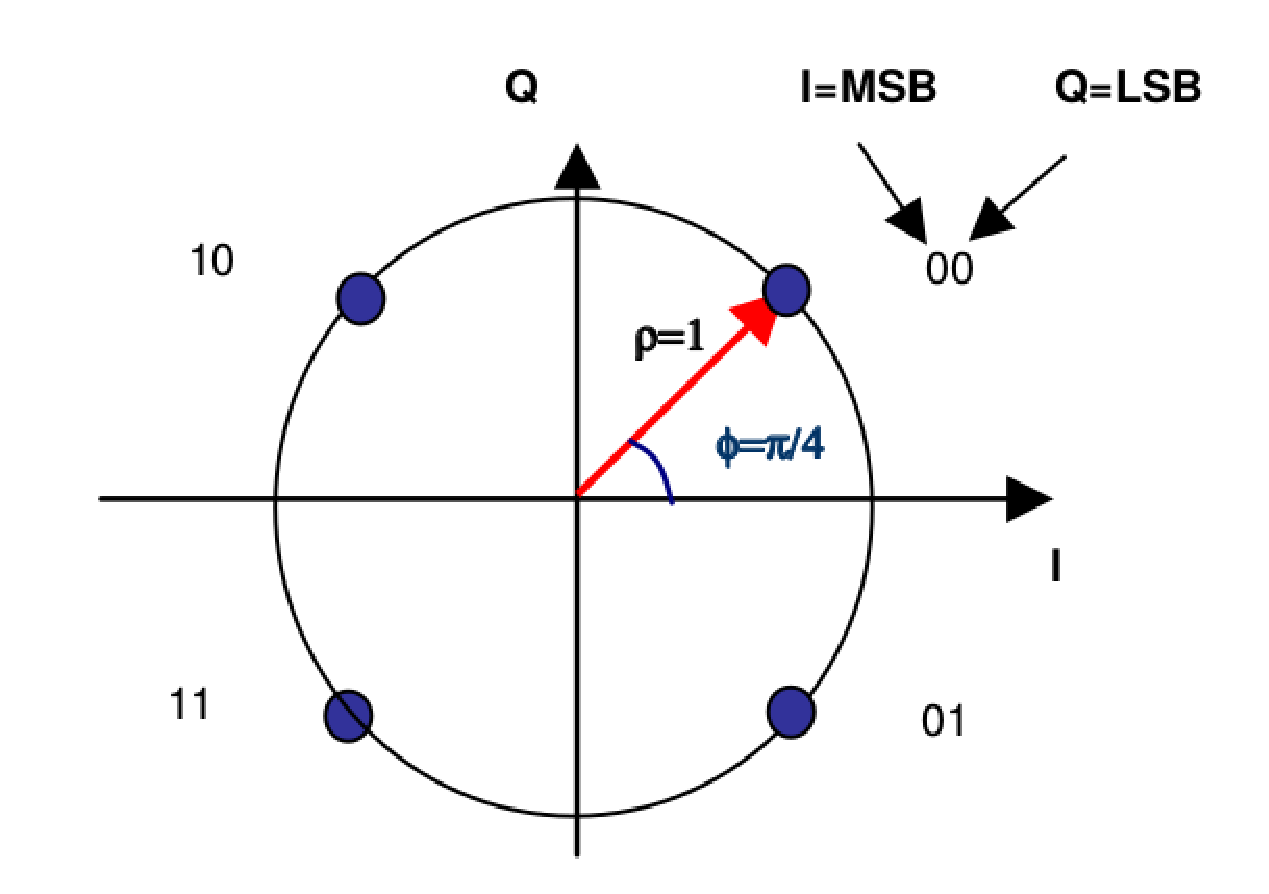
\includegraphics[width=\columnwidth]{./figs/qpsk}
\caption{Constellation Diagram of QPSK}
\label{fig : qpsk}
\end{center}
\end{figure}
\subsection{Approximated LLR's for 8-PSK Mapping Scheme}
For the 8-PSK mapping scheme showed in Fig. \ref{fig : 8psk} is grey code constellation and  $b_2,b_0$ are the MSB and LSB of the mapped symbols.
\begin{align}
LLR(b_2)&\approx \max \brak{L_0,L_1,L_3,L_2} -\max \brak{L_6,L_7,L_5,L_4} \\
LLR(b_1)&\approx \max \brak{L_0,L_1,L_5,L_4} -\max \brak{L_3,L_2,L_6,L_7}\\
LLR(b_0)&\approx \max \brak{L_0,L_2,L_6,L_4} -\max \brak{L_1,L_3,L_7,L_5}
\end{align}
Where,
\begin{align}
L_i = e^{-\frac{\abs{y-x_i}^2}{2\sigma^2}} \quad i=0,1,\dots,7
\end{align}
\begin{figure}[!ht]
\begin{center}
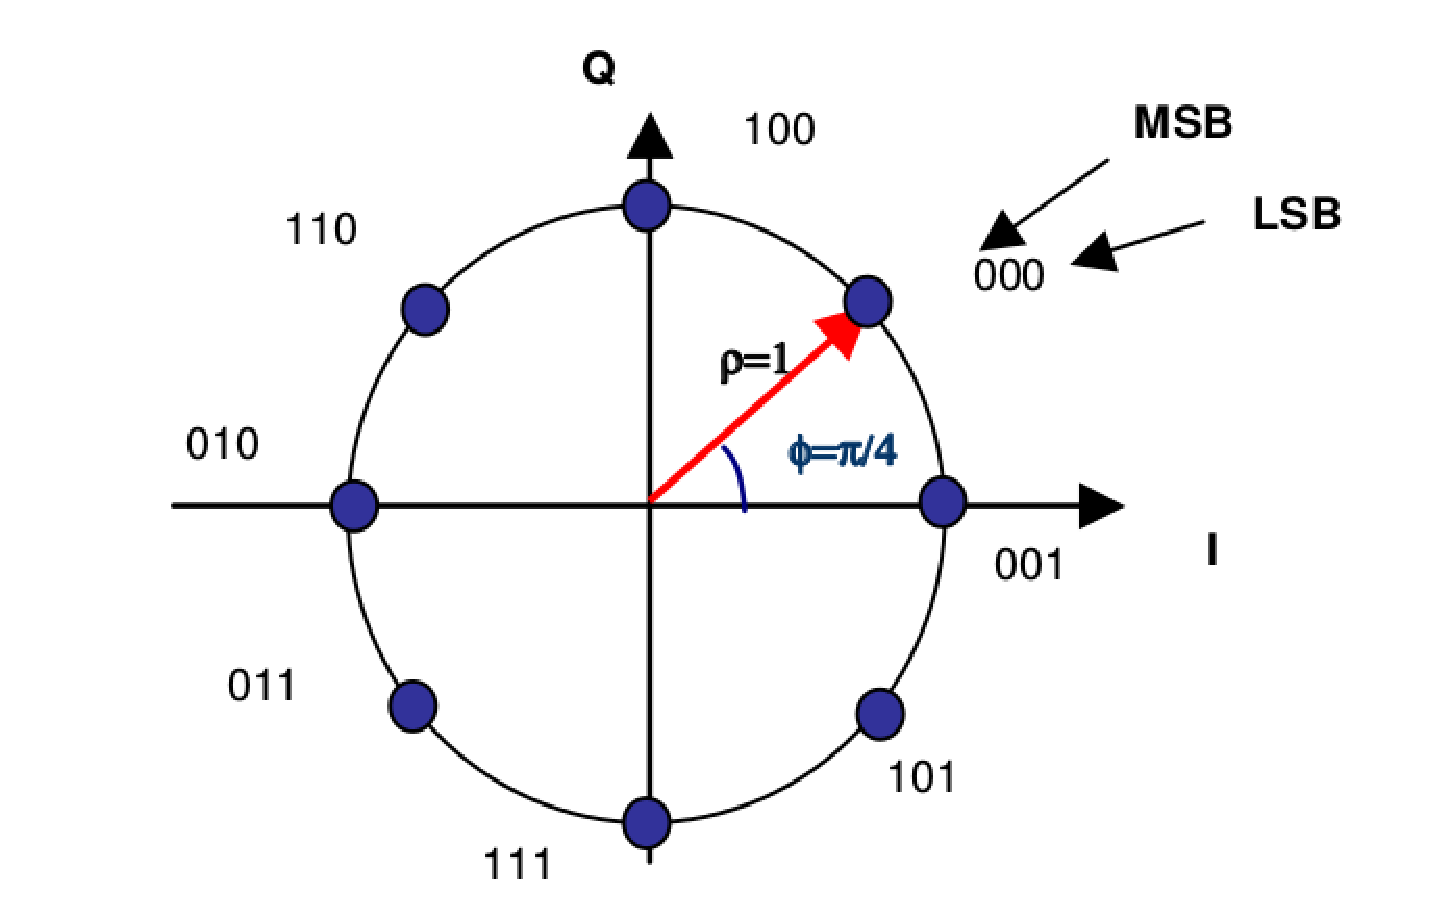
\includegraphics[width=\columnwidth]{./figs/8psk}
\caption{Constellation Diagram of 8-PSK}
\label{fig : 8psk}
\end{center}
\end{figure}


\section{Carrier Synchronization}
\subsection{Time Offset: Gardner TED}
%\subsection{Transmitter}
%\begin{equation}
%m \rightarrow\boxed	{BPSK}\rightarrow\boxed	{\uparrow T_{sym}}\rightarrow C	
%\end{equation}
%
%  Let bit stream was $m$, $xc$ will be mapped sequence and $C$ will be upsampled by $T_{sym}$
% Where $T_{sym}$ is the samples per symbol. 
%\begin{equation}
%X=P \circledast C
%\end{equation} where $P$ is the shape of the pulse. And defined as,
%\begin{equation}
%    P =
%    \begin{cases}
%      1 & 0\leq t\leq 99 \\
%      0        & otherwise
%    \end{cases}
%  \end{equation}
%\subsection{Receiver}
Let the $m$th sample in the $r$th received symbol time slot be
\begin{equation}
Y_k(m)= X_k + V_k(m), \quad k = 1,\dots,N, m = 1 ,\dots,M.
\end{equation} 
where $X_k$ is the transmitted symbol in the $k$th time slot and $V_k(m) \sim \mathcal{N}\brak{0,\sigma^2} $. 
The decision variable for the $k$th symbol 
is 
\cite{time_offset}
%\begin{align}
%U_k&=Y_{k-1}\brak{\frac{M}{2}}\sbrak{Y_{k}\brak{M}-Y_{k-1}\brak{M}}
\begin{align}
U_k=\frac{1}{N}\sum^{N}_{i=1}Y_{k-i}\brak{\frac{M}{2}}\sbrak{Y_{k-i+1}\brak{M}-Y_{k-i}\brak{M}}
\end{align}
%\end{align}
%

\subsection{Frequency Offset: LR Technique}
%There are two parts.
%\begin{itemize}
%\item Estimate
%\item Exact
%\end{itemize}
Let the frequency offset be 
$\Delta f$  
\cite{freq_offset}
.  Then
\begin{equation}
\label{eq:freq_offset_model}
Y_k= X_k e^{j2\pi\Delta fkM} + V_k, \quad k = 1,\dots,N 
\end{equation}  
From \eqref{eq:freq_offset_model},
%
\begin{align}
Y_kX_k^*&= \abs{X_k}^2e^{j2\pi\Delta fkM}+ X_k^*{V}_k\\
\implies r_k&=e^{j2\pi\Delta fkM}+ \bar{V}_k
\end{align}
where
\begin{align}
r_k=Y_kX_k^*, \bar{V}_k=X_k^*{V}_k, \abs{X_k}^2=1
\end{align}
%
The autocorrelation can be calculated as
\begin{equation}
R(k) \overset{\Delta}{=} \frac{1}{N-k}\sum_{i=k+1}^{N} r_{i}r^{*}_{i-k}
 , 1 \leq k \leq N-1
\end{equation}
Where N is the length of the received signal.
%DVB-S2 operating with large frequency. So Large frequency offset model has to be employed which is the  Exact approximation of LR technique \cite{1}
For large centre frequency, the following yields a good approximation for frequency offset upto 40 
MHz.
\begin{equation}
\Delta\hat{f} \approx \frac{1}{2\pi M}\frac{\sum_{k=1}^{P}\text{Im}(R(k))}{\sum_{k=1}^{P}k\text{Re}(R(k))},
\quad  P\Delta{f}M << 1
\label{eq:Z}
\end{equation}
%
where $P$ is the number of pilot symbols.


\subsection{Phase Offset: Feed Forward Maximum Likelihood (FF-ML)technique}
%There are two parts.
%\begin{itemize}
%\item Estimate
%\item Exact
%\end{itemize}
Let the phase offset be 
$\Delta\phi$  
\cite{phase_offset}
.  
Then for the $k$th pilot,
\begin{equation}
\label{eq:phase_offset_model}
Y_k= X_k e^{j\Delta\phi_k} + V_k, \quad k = 1,\dots,P
\end{equation}  
From \eqref{eq:phase_offset_model},
%
\begin{align}
Y_kX_k^*&= \abs{X_k}^2e^{j \Delta\phi_k}+ X_k^*{V}_k\\
\implies r_k&=e^{j\Delta\phi_k}+ \bar{V}_k
\label{eq:rk}
\end{align}
where
\begin{align}
r_k=Y_kX_k^*, \bar{V}_k=X_k^*{V}_k, \abs{X_k}^2=1
\end{align}
From \eqref{eq:rk}, the estimate for the $k$th pilot is obtained as
%$\hat{\phi}$ can be written as: 
\begin{equation}
\label{eq:phase_estimation}
\Delta\hat{\phi}_k  = \arg\brak{r_k}
\end{equation} 
%
The phase estimate is then obtained using $\Delta\hat{\phi}_k $ in the following update equation as
\begin{equation}
\Delta\theta_k =\Delta\theta_{k-1} + \alpha{SAW}\sbrak{\Delta\hat{\phi}_k
-\Delta\theta_{k-1}}
\end{equation}
%
Where $SAW$ is sawtooth non-linearity 
\begin{equation}
 SAW[\phi]=\sbrak{\phi}^{\pi}_{-\pi}
\end{equation} 
and $\alpha \leq 1$. The estimate is then obtained as $\Delta\theta_{P}$.
%\\$l$ counts the 
%number of pilot-based estimates.\\ ${\hat{\Delta\phi}^{(p)}}_{f}(l)$  is the final unwrapped pilot estimate.
 
\subsection{Automatic Gain Controller (AGC): Data-Aided Vector-Tracker (DA-VT) }
Let the random AGC offset $\alpha$, then the received symbol equation with amplitude offset as,
\begin{equation}
\label{eq:AGC model}
Y_k = \alpha X_k +V_k  \quad k = 1,\dots,P
\end{equation}
%
where $\alpha = \alpha_I+j\alpha_Q$ is the gain parameter.
According to \cite{agc}, the $\hat{\alpha_k}$ estimate for the $k$th pilot is
%
\begin{equation}
\alpha_{k+1}=
%\begin{cases}
\alpha_k-\gamma\sbrak{\alpha_k Y^p_k - X^p_k}\sbrak{X^p_k}^*, 
%& k \in pilot symbols \\
%\alpha_k, & otherwise
%\end{cases}
\end{equation}
%
where $\gamma$ is the AGC step size.
%\begin{align}
%\alpha_{k+1}=\alpha_k + \mu \Delta J
%\end{align}
%Where ,
%\begin{equation}
%\Delta J=\brak{{\sbrak{\abs{Re(\hat{s(k)})}-\alpha_k\abs{Re(z(k)}}
%+\sbrak{\abs{Im(\hat{s(k)})}-\alpha_k\abs{Im(z(k)}}}}
%\end{equation}
%
\section{Frame Synchronization : Global Summation of SOF/PLSC Detectors} 
%
%
Let the frequency offset be $\Delta f$ and phase offset be $\Delta \phi$.Then,
\begin{equation}
%\label{eq:freq_offset_model}
Y_k= X_k e^{j(2\pi\Delta fkM+\phi_k)} + V_k, \quad k = 1,\dots,N 
\end{equation}
%
assuming that no pilot symbols are trasmitted. 
Let the phase information be $\theta_k$, and defined as
%
\begin{equation}
\theta(k) = \frac{Y_k}{\abs{Y_k}}
\end{equation}
%
At the receiver, the header information is available in the form of 
\begin{align}
g_i(l)&=x_s(l)x_s(l-i), l = 0,\dots, SOF-1
\\
h_i(l)&=x_p(l)x_p(l-i), l = 0,\dots, PLSC-1
\end{align}
%
where $x_s$ are the mapped SOF symbols, $x_p$ are the scrambled PLSC  symbols, both  modulated using $\pi/2$ BPSK
for $i=1,2,4,8,16,32$.
A special kind of correlation is performed to obtain
\begin{align}
m_i(k)&=\sum_{l=0}^{PLSC-1} e^{j(\theta(k-l)-\theta(k-l-i))} h_i(l),
\\
n_i(k)&=\sum_{l=0}^{SOF-1} e^{j(\theta(k-l)-\theta(k-l-i))} g_i(l) ,
\\
&k = 1, \dots, N 
\end{align}
%
Compute
\begin{align}
p_i(k)=
\begin{cases}
\max \lbrak{\abs{n_i({k-PLSC})+m_i(k)},} &
\\
\rbrak{\abs{n_i({k-PLSC})-m_i(k)}} & k > PLSC
\\
\max \abs{m_i(k)}  & k < 64
\end{cases}
\end{align}

 GLOBAL variable $G_{R,T}(k)$  \cite{frame_offset} defined as,

\begin{equation}
G_{R,T}(k)=\sum_{i\geq1}p_i(k) , \quad i=1,2,4,8,16,32
\label{eq:global}
\end{equation}

At the receiver, let us consider we have sent two types of transmission. One is PLHEADER+DATA $\brak{Y_{k1}}$ and another is only DATA $\brak{Y_{k2}}$ and the GLOBAL variables for $\brak{Y_{k1}}$ and $\brak{Y_{k2}}$ from \eqref{eq:global} are $G1_{R,T}(k)$, $G2_{R,T}(k)$ respectively.

\subsection{Global Threshold Calculation}
The Global Threshold variable is defined as
\begin{align}
T&= \max \brak{ \max \brak{G1_{R,T}(k)},\max \brak{ G2_{R,T}(k)}}
\end{align} 
%\subsection{False Alarm Probability}
The probability of false detection of plheader when only DATA frame $\brak{Y_{k2}}$ has been sent is defined as
\begin{align}
P_{FA} &= \frac{\sum \frac{sign(\abs{Y_{k2}-T})+1}{2} }{N}
\end{align}

%\subsection{Missed Detection Probability}
The probability of missed detection of plheader when PLHEADER+DATA $\brak{Y_{k1}}$ has been sent is defined as
\begin{align}
P_{MD} &= \frac{\sum \frac{sign(T-\abs{Y_{k1}})+1}{2} }{N+PLSC+SOF}
\end{align}
%\subsection{False Alarm Probability}
%False Alarm Probability $(p_{fa})$, is the probability of false detection of plheader when only DATA frame has been sent.
%%\subsection{Missed Detection Probability}
%Missed Detection Probabililty $(p_{md})$, is the probability of missed detection of plheader when PLHEADER+DATA has been sent.



%
%\begin{thebibliography}{20}
%\bibitem{1}
%U. Mengali and A. N. D'Andrea:'synchronization Techniques for Digital Receivers,' New York: Plenum, 1997.
%
%\bibitem{2}
%F. M. Gardner:'A BPSK/QPSK timing-error detector for sampled receivers,' IEEE TRANSACTIONS ON COMMUNICATIONS, VOL.COM-34,NO.5,MAY 1986
%\bibitem{3}
%M. Luise and R. Reggiannini:'Carrier frequency recovery in all-digital modems for burst mode transmissions,' IEEE Trans. Commun., vol. 43,
%no. 2/3/4, pp. 1169-1178, Feb/Mar/Apr 1995.
%
%\bibitem{4}
%E. Casini, R. De Gaudenzi, and A. Ginesi:'DVB-S2 modem algorithms
%design and performance over typical satellite channels,' International
%Journal of Satellite Communications and Networking 2004, vol. 22(3), pp. 281-318, 2004.
%
%
%\end{thebibliography}

\section{Results and Discussion}
\subsection{Time Offset}
Fig. \ref{fig:8psk1} Shows the Simulation diagram.  Fig. \ref{fig:qpsk1} Shows the Simulation diagram.
%
\begin{figure}[!ht]
\begin{center}
\includegraphics[width=\columnwidth]{./figs/8PSK1}
\end{center}
\caption{SNR vs BER for 8-PSK}
\label{fig:8psk1}
\end{figure}
\begin{figure}[!ht]
\begin{center}
\includegraphics[width=\columnwidth]{./figs/8PSK1}
\end{center}
\caption{SNR vs BER for 8-PSK}
\label{fig:8psk1}
\end{figure}
\begin{figure}[!ht]
\begin{center}
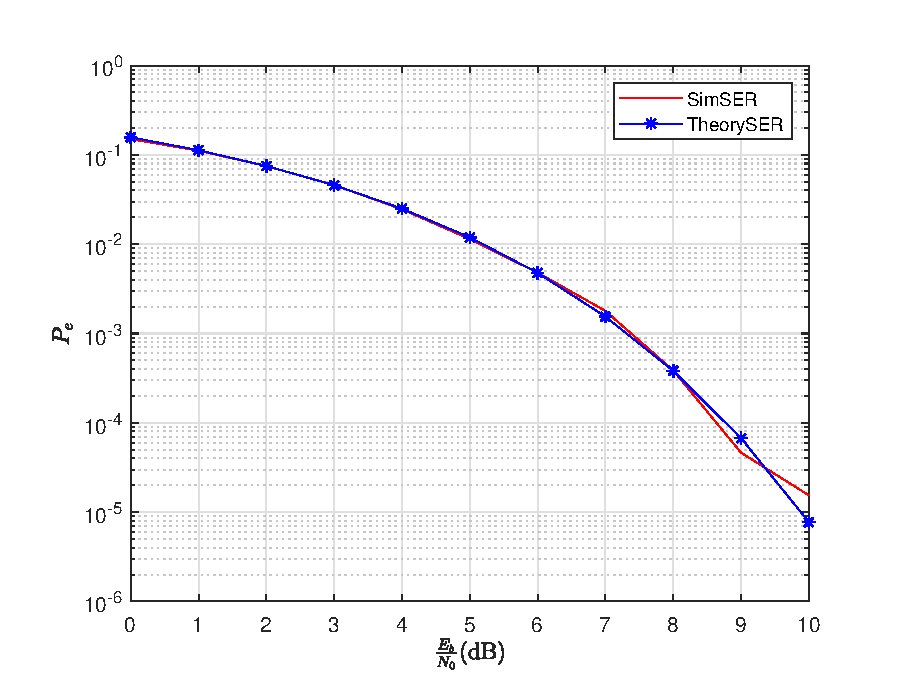
\includegraphics[width=\columnwidth]{./figs/QPSK1}
\end{center}
\caption{SNR vs BER for QPSK}
\label{fig:qpsk1}
\end{figure}
\begin{figure}
\begin{center}
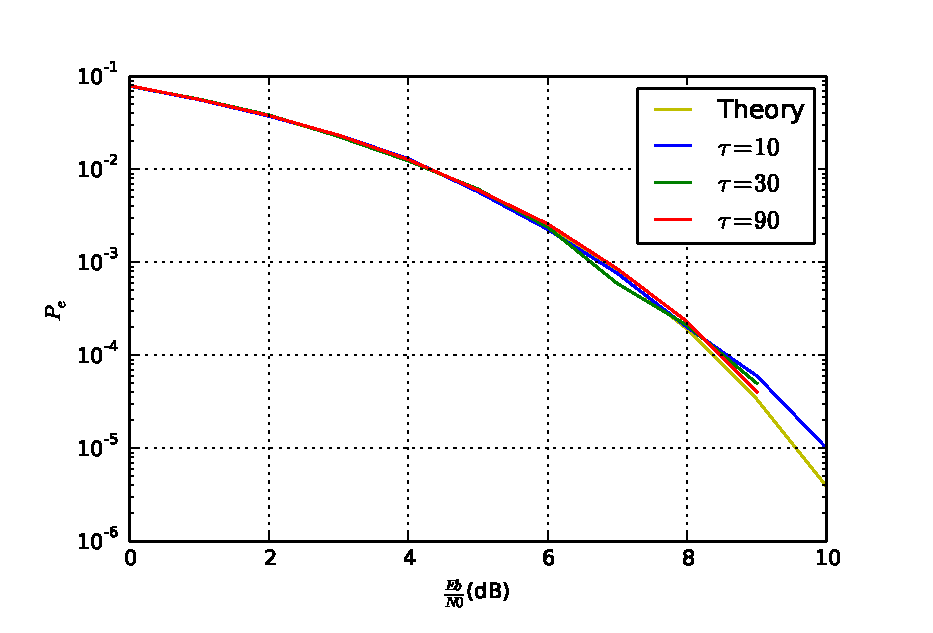
\includegraphics[width=\columnwidth]{./figs/Different_timeoffsets_snrvsber.eps}
\end{center}
\caption{SNR vs BER for varying $\tau$.}
\label{fig:difftoff}
\end{figure}
%
%\begin{figure}
%\begin{center}
%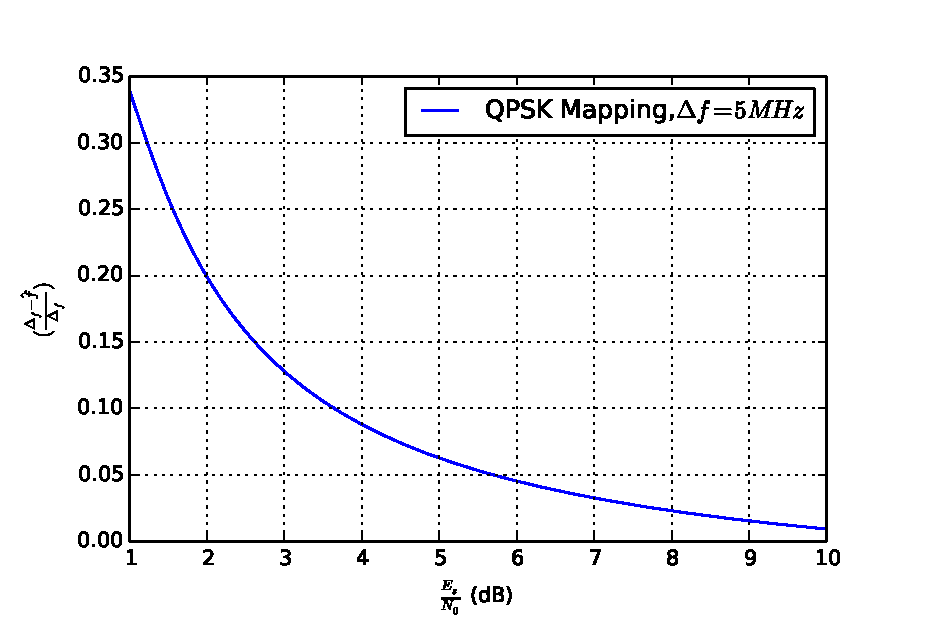
\includegraphics[width=\columnwidth]{./figs/frequencyestiamtion_best_error_vs_snr.eps}
%\end{center}
%\caption{$\Delta f = 5$ MHz}
%\label{fig:freq_est}
%\end{figure}

%
Fig. \ref{fig:difftoff} is generated by the following code
\begin{lstlisting}
https://github.com/gadepall/EE5837/raw/master/synctech/codes/time_sync_offsets.py
\end{lstlisting}
and shows the variation of the BER with respect to the SNR  with 
different timing offsets $\tau$ for $N = 6$.
%$\Delta f$ when the SNR = 10 dB. 
% Similarly Fig. \ref{fig:difftoff} shows the variation of the error with 
%respect 
%to the SNR .
\subsection{Frequency}
\begin{figure}
\begin{center}
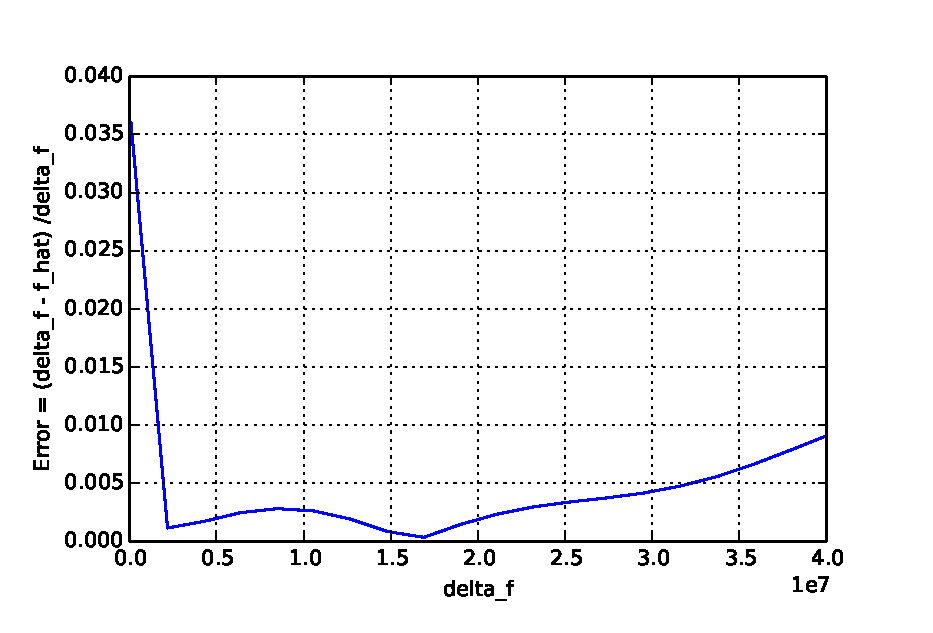
\includegraphics[width=\columnwidth]{./figs/frequency_best.eps}
\end{center}
\caption{Error variation with respect to frequency offset.  }
\label{fig:freq_best}
\end{figure}
%
\begin{figure}
\begin{center}
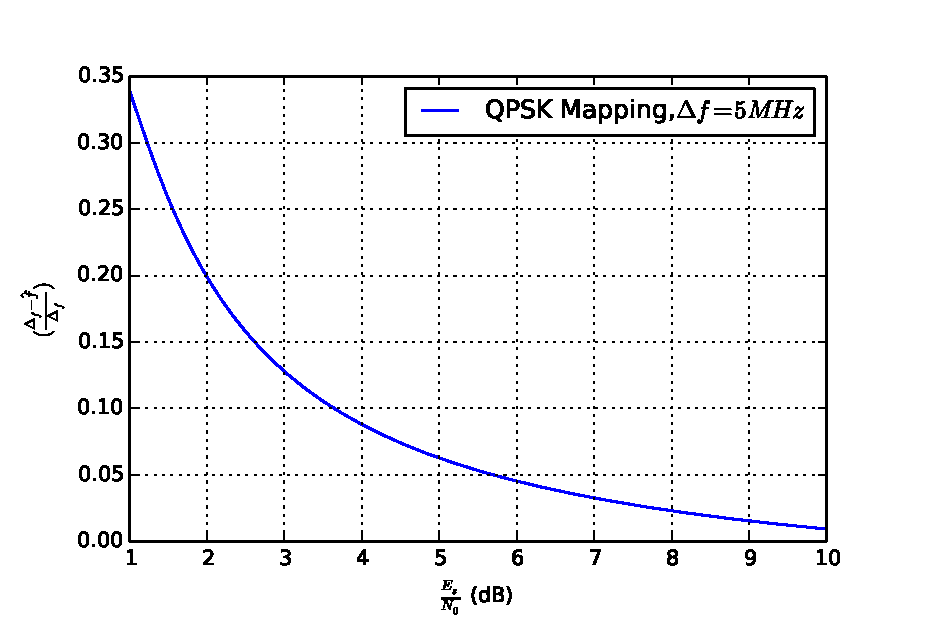
\includegraphics[width=\columnwidth]{./figs/frequencyestiamtion_best_error_vs_snr.eps}
\end{center}
\caption{Error variation with respect to the SNR.  $\Delta f = 5$ MHz, Center frequency $f_c=25$ GHz}
\label{fig:freq_est}
\end{figure}

%
The number of pilot symbols is $P = 18$. The codes for generating the plots are available at

Fig. \ref{fig:freq_best} shows the variation of the error in the offset estimate with respect to the offset 
$\Delta f$ when the SNR = 10 dB.  Similarly Fig. \ref{fig:freq_est} shows the variation of the error with 
respect 
to the SNR for $\Delta f = 5 $MHz.
\subsection{Plots}
Fig. \ref{fig:phaseerrorp} is generated using 
\begin{lstlisting}
https://github.com/gadepall/EE5837/raw/master/synctech/codes/Error_vs_lp.py
\end{lstlisting}
and  shows the variation of the phase error in the offset estimate with respect to the pilot symbols  when the 
SNR = 10 dB and $\alpha = 0.5$.

\begin{figure}[!ht]
\begin{center}
\includegraphics[width=\columnwidth]{./figs/Phase_error_with_respect_to_pilots.eps}
\end{center}
\caption{Phase error variation with respect to pilot symbols }
\label{fig:phaseerrorp}
\end{figure}
%
Similarly Fig. \ref{fig:phaseerrorsnr} generated by 
\begin{lstlisting}
https://github.com/gadepall/EE5837/blob/master/synctech/codes/Error_vs_snr.py
\end{lstlisting}
shows the variation of the error with 
respect 
to the SNR for pilot symbols $P = 18$ and  $\alpha = 1$.

\begin{figure}[!hb]
\begin{center}
\includegraphics[width=\columnwidth]{./figs/Phase_error_with_respect_to_SNR_fixed_pilot.eps}
\end{center}
\caption{$\Delta f = 5$ MHz}
\label{fig:phaseerrorsnr}
\end{figure}
%
\subsection{Plots}
%
%\begin{figure}
%\begin{center}
%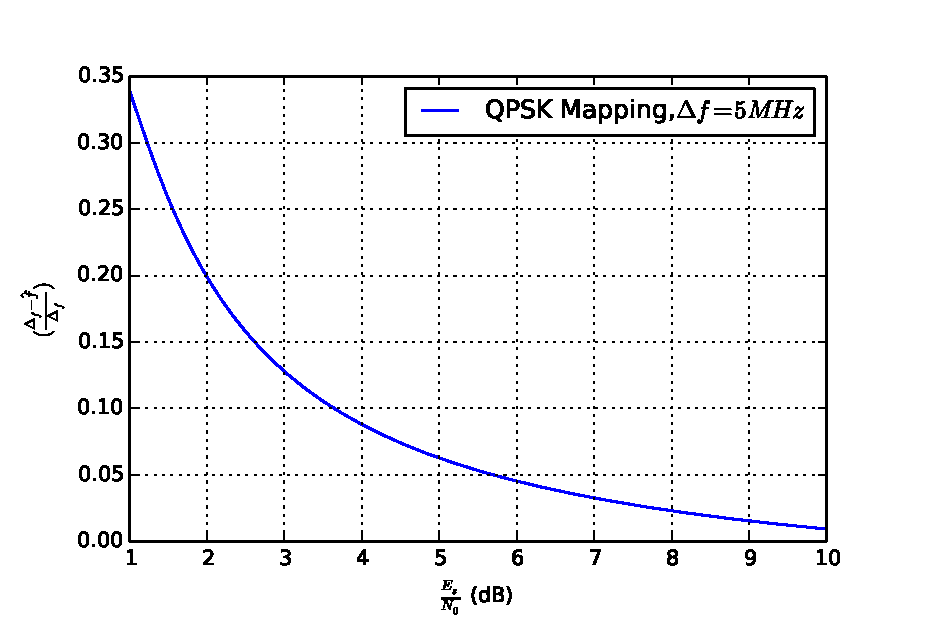
\includegraphics[width=\columnwidth]{./figs/frequencyestiamtion_best_error_vs_snr.eps}
%\end{center}
%\caption{$\Delta f = 5$ MHz}
%\label{fig:freq_est}
%\end{figure}

%
The following code plots the real and imaginary parts of the gain parameter $\alpha$ with respect to the number of pilot symbols $P$.
in Fig. \ref{fig:diffaoff}.  $\gamma = 10^{-3}, SNR=10 dB$.

%
\begin{figure}[!ht]
\begin{center}
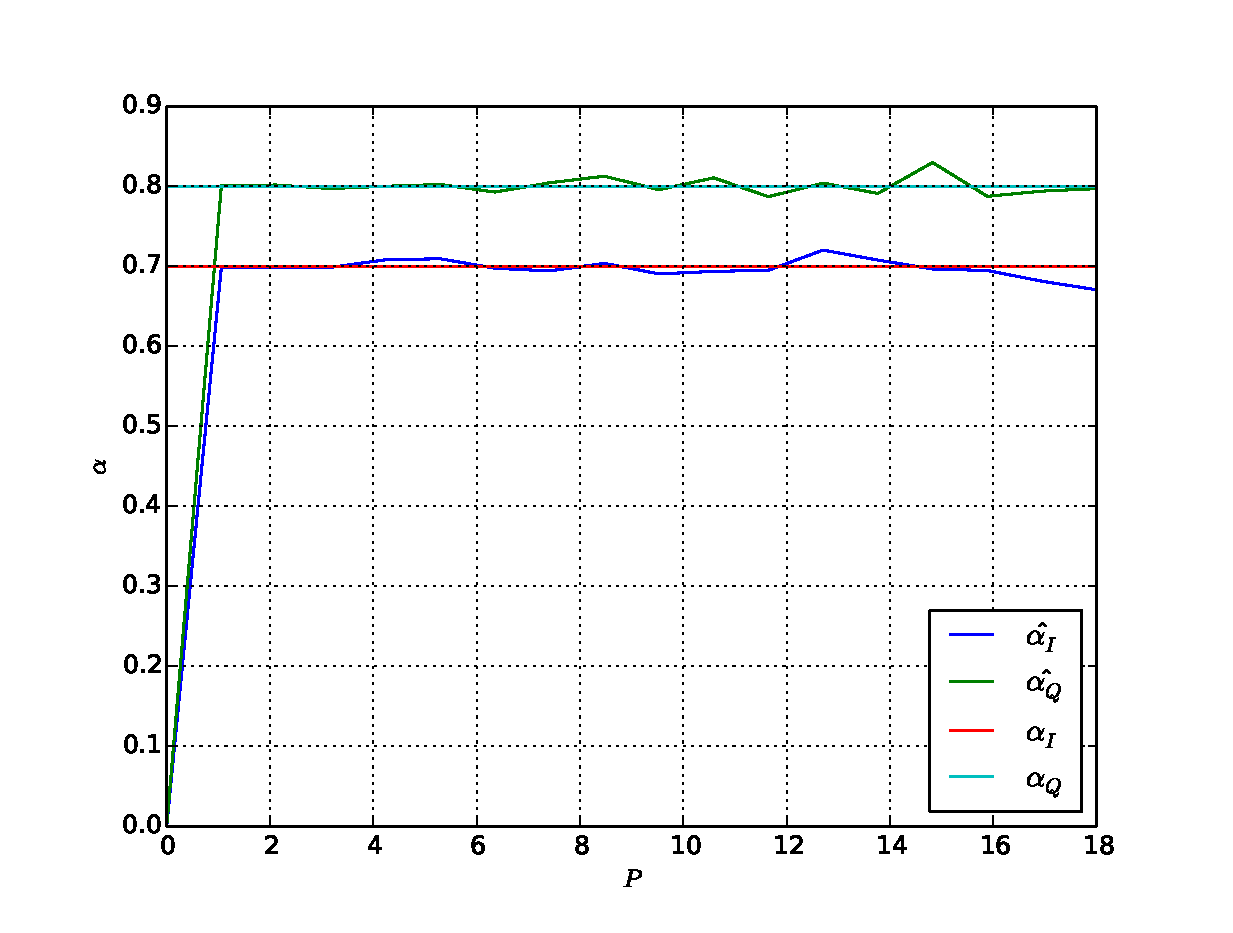
\includegraphics[width=\columnwidth]{./figs/Convergence_of_Digital_AGC.eps}
\end{center}
\caption{Convergence of Digital AGC with resepct to P.}
\label{fig:diffaoff}
\end{figure}

\begin{lstlisting}
https://github.com/gadepall/EE5837/raw/master/synctech/codes/Digital_AGC_with_fixed_SNR.py
\end{lstlisting}
%\bibliography{IEEEabrv,./bib/ldpc.bib}
%\bibliography{IEEEabrv,Theresh_timesync.bib}
\subsection{Frame}

\begin{figure}[!ht]
\begin{center}
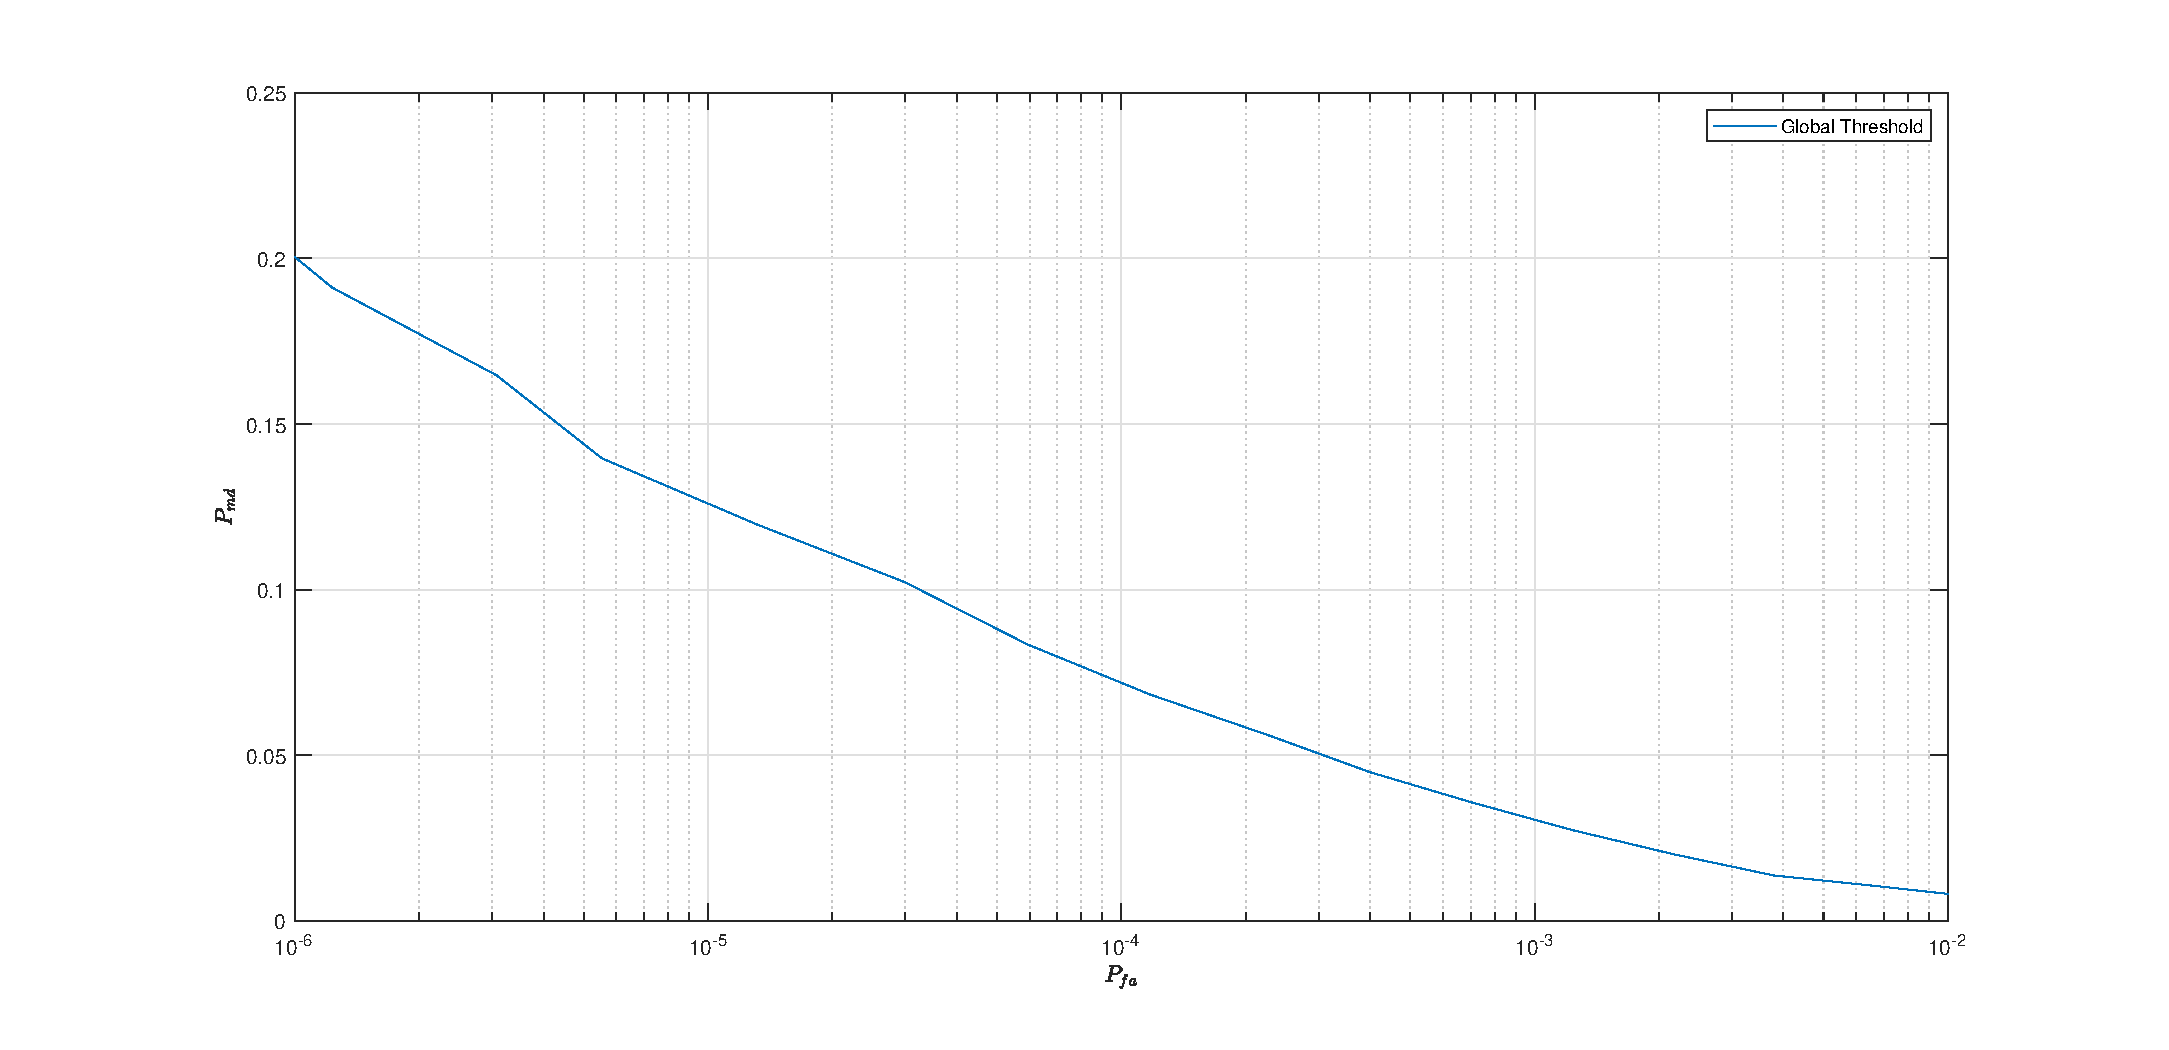
\includegraphics[width=\columnwidth]{./figs/framesync.eps}
\end{center}
\caption{Frame Synchronization Receiver Operating Characteristcs (ROC)}
\label{fig:frameoff}
\end{figure}

Fig.\ref{fig:frameoff} shows the ROC curve ($P_{FA} vs P_{MD}$)  at the receiver for frame synchronization at $\frac{E_b}{N_0}=-2$ dB.
\bibliography{IEEEabrv,dvbs2.bib}

\end{document}

